\chapter{Agorà: proposed framework}\label{agora}

\lettrine{C}{hapter} 5 shows technical implementation of the proposed framework, dividing the overall workflow in all possible use cases; in the last part, a sketch application explains how tesiCris client module is integrated and how it works.


\section{Introduction}

tesiCris implements all possible situations that can happen in a scenario as the one described in the previous chapter (\ref{methodology}).

The MQTT protocol (\cite{banks2014mqtt}) makes possible all the communications among components: tesiCris uses Eclipse Paho MQTT Python Client and Eclipse Paho MQTT C Client for managing messages exchange (\cite{o2014paho}), while it uses Eclipse Mos\-quitto as broker (\cite{light2013mosquitto}). The Machine Learning library MLlib by Apache Spark\textsuperscript{TM} (\cite{spark2015apache}) is used to predict the applications complete models.

The next technical use cases implementation makes use of application \textit{Swaptions} as reference, taken from the PARSEC benchmark suite (\cite{bienia2008parsec}). This application is a workload which prices a portfolio of swaptions through Monte Carlo simulations; it has two tunable parameters, the number of threads (variable \textit{num\_threads}, from 1 to 8) and the number of trials for the simulation (variable \textit{num\_trials}, from 100.000 to 1.000.000 with a step of 100.000), while metrics of interest are throughput (variable \textit{avg\_throughput}), as the number of priced swaptions per second, and error (variable \textit{avg\_error}), computed as:

\[
avg\_error = \dfrac{\sum_{s \in pricedSwaptions} \left\vert StandDevRef(s) - StandDev(s) \right\vert}{\left\vert pricedSwaptions \right\vert}
\]

where $StandDevRef(s)$ is the reference standard deviation for swaption $s$, $StandDev(s)$ is the evaluated one and $pricedSwaptions$ represents all swaptions that are priced every computing cycle; so, metric $avg\_error$ stands for the average of differences between standard deviation of priced swaptions using evaluated configuration with respect to the reference one (standard deviation for 1.000.000 trials).

tesiCris has been interconnected to the mARGOt autotuner (\cite{gadioli2015application}), that exploits design-time knowledge to dynamically adapt applications behavior during execution; mARGOt represents this information as a list of Operating Points (OPs): an OP is made by a set of parameters values, also called software knobs, in union with the associated performance (metrics of interest values), profiled at design-time; tesiCris improvement is to build application knowledge at runtime, with an online distributed Design Space Exploration phase in which a subset of OPs are collected, in order to predict the complete model, made by the entire Operating Point list.

tesiCris could work in union with other autotuners that, using application knowledge in terms of configurations and associated performances, have the capability to dynamically adapt applications behavior during execution.










\section{Use case implementation}





\subsection{server\_listener module creation}

The starting point is the creation of the server\_listener module, that is in charge of managing the arrival of applications; it connects to the MQTT broker and it subscribes to topic "tesiCris/apps":

\begin{figure}[H]

    \centering
    
\includegraphics[width = \textwidth]{server_listener_subscription}
    \caption{server\_listener subscription}
    
\end{figure}





\subsection{Application arrival}

An application can be already known by the server\_listener module or a program is executed by a machine for the first time.

\subsubsection{Unknown application}

A node starts running a program; the related client module notifies this event, publishing on topic "tesiCris/apps" a string composed of the application name and the machine hostname plus the Process IDentifier (PID), with format "\textit{[appName] [hostname]\_[PID]}", so that the client can be univocally recognized in the future; the message is dispatched to the server\_listener, that creates a dedicated server\_handler for that application:

\begin{figure}[H]

    \centering
    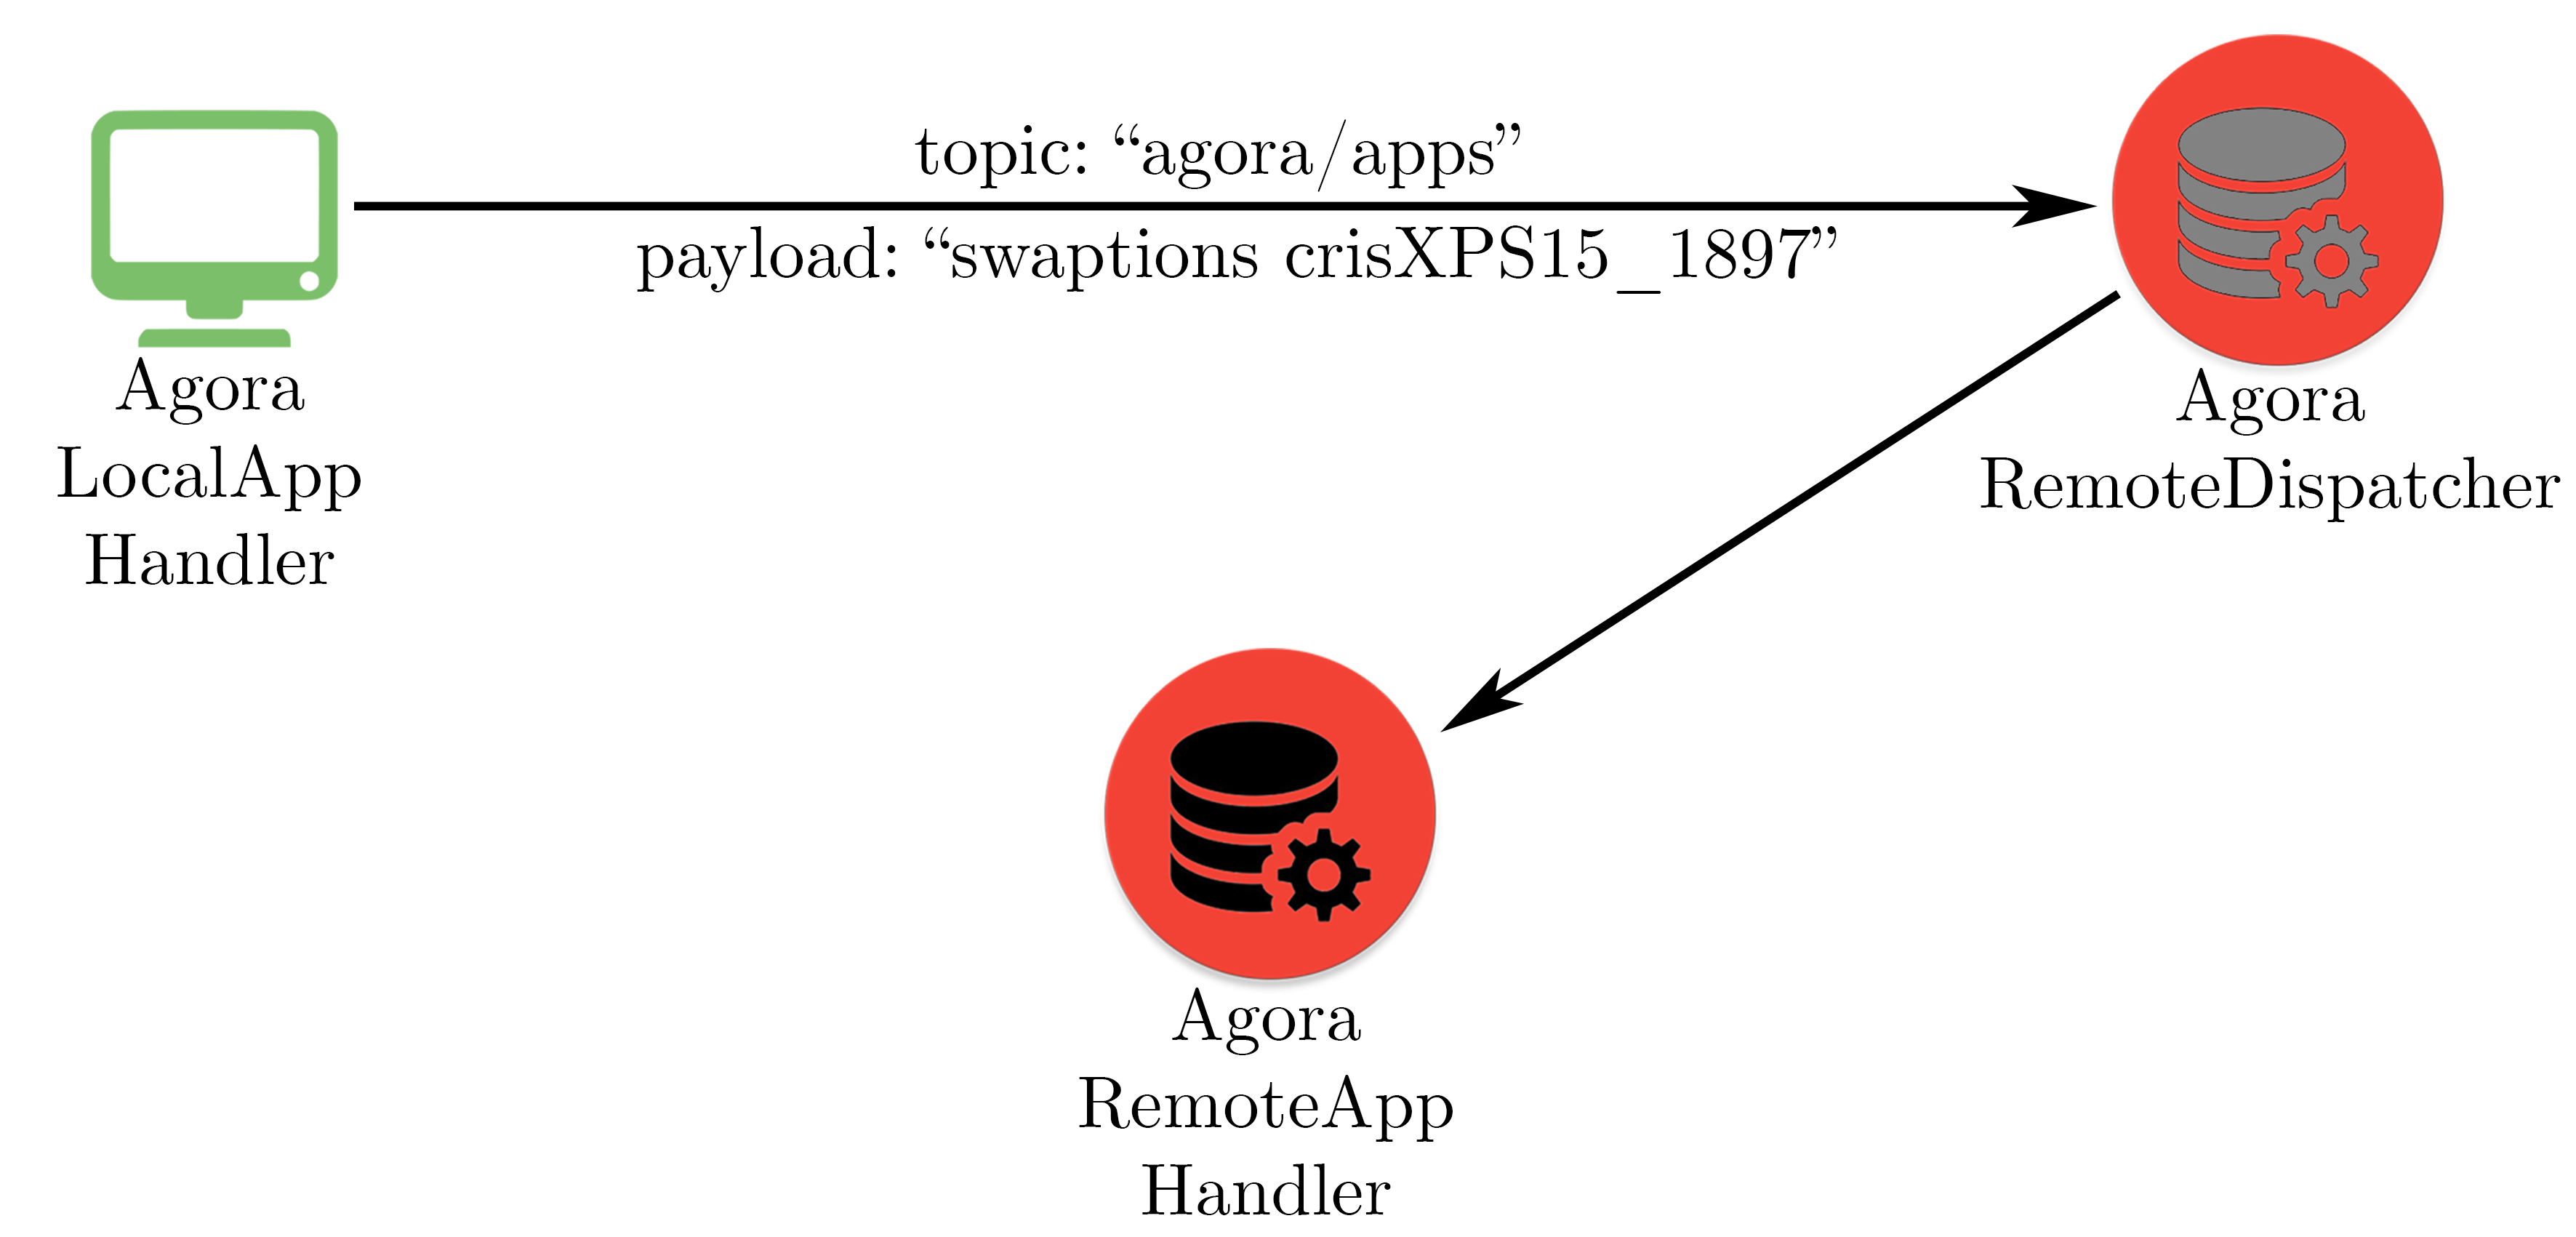
\includegraphics[width = \textwidth]{new_unknown}
    \caption{New unknown application arrival example; a dedicated ser\-ver\_handler is created by the server\_listener}
    
\end{figure}

At the beginning, the client module subscribes to some topics that are needed to receive communications from the related server\_handler:

\begin{enumerate}

    \item "tesiCris/\textit{[appName]}", in order to understand if the server\_handler has asked application information and, therefore, to reply (see \ref{req_info}); this topic is also used to understand if the server\_handler has crashed and, so, to react properly (see \ref{handler_disc});
    
    \item "tesiCris/\textit{[appName]}/\textit{[hostname]\_[PID]}/conf", in order to receive configurations from the server\_handler during Design Space Exploration phase (see \ref{dse_conf});
    
    \item "tesiCris/\textit{[appName]}/\textit{[hostname]\_[PID]}/model", in order to receive\linebreak a partial OP list (see \ref{DoEModelSend}) and the complete predicted model from the server\_handler (see \ref{modelSend}).

\end{enumerate}

\begin{figure}[H]

    \centering
    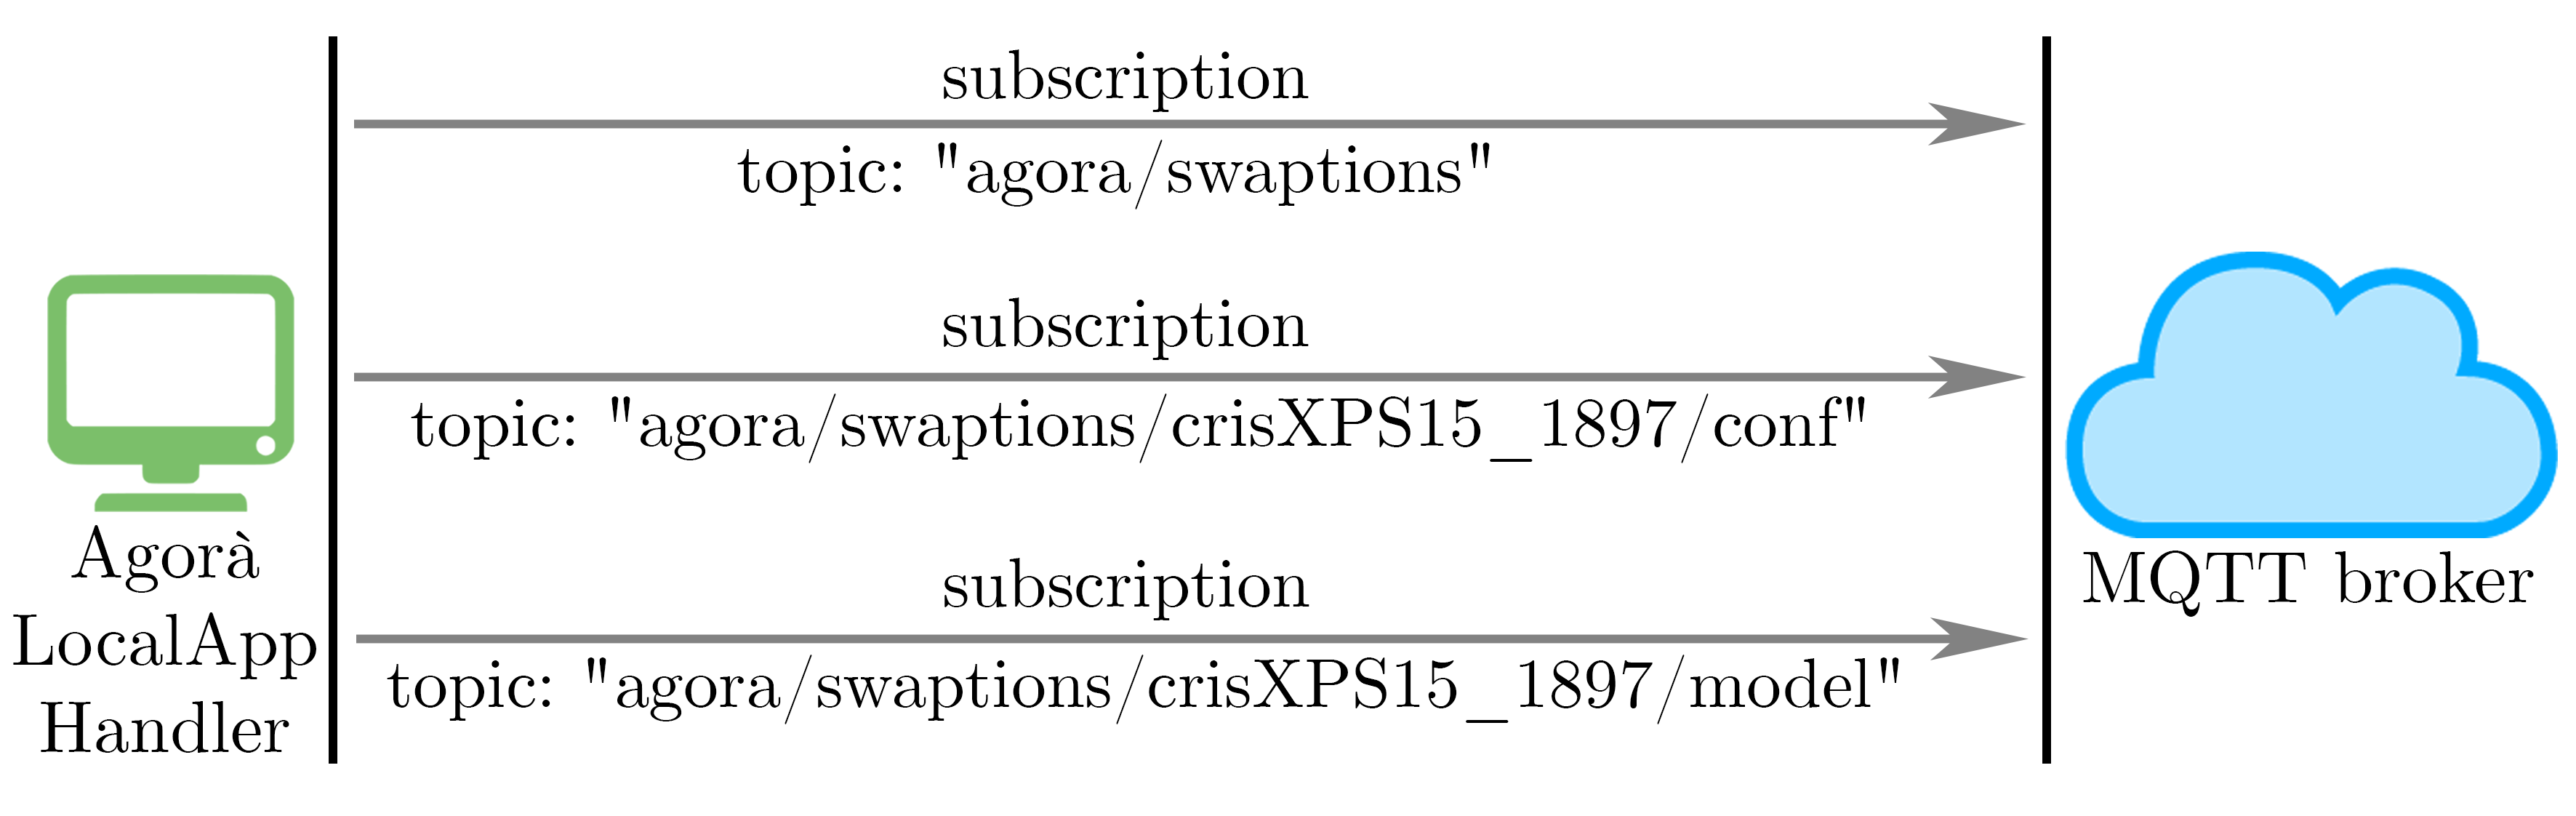
\includegraphics[width = \textwidth]{client_subs}
    \caption{client MQTT subscriptions example}
    
\end{figure}

The server\_handler subscribes to some topics in order to manage correctly all the various situations that happens:

\begin{enumerate}

    \item "tesiCris/\textit{[appName]}/newHostpid", in order to manage the hypothetical arrival of other clients that are running the supervised application (see \ref{knownApp});
    
    \item "tesiCris/\textit{[appName]}/req", in order to manage all the requests made by clients during program execution (see \ref{clientReq});
    
    \item "tesiCris/\textit{[appName]}/info/\#", in order to receive all the available application information, such as parameters name and values (see \ref{client_info}); the real topic will be with format "tesiCris\slash{}\textit{[appName]}\slash{}info\slash{}\textit{[host\-name]\_ [PID]}", therefore the server\_handler can store the ID of the node that is sending application information, in order to react properly to a possible client crash during this phase (see \ref{client_disc});
    
    \item "tesiCris/\textit{[appName]}/disconnection", in order to correctly react to a possible node disconnection (see \ref{client_disc});
    
    \item "tesiCris/\textit{[appName]}/OPs", in order to receive Operating Points from clients during Design Space Exploration phase (see \ref{opSend}).

\end{enumerate}

\begin{figure}[H]

    \centering
    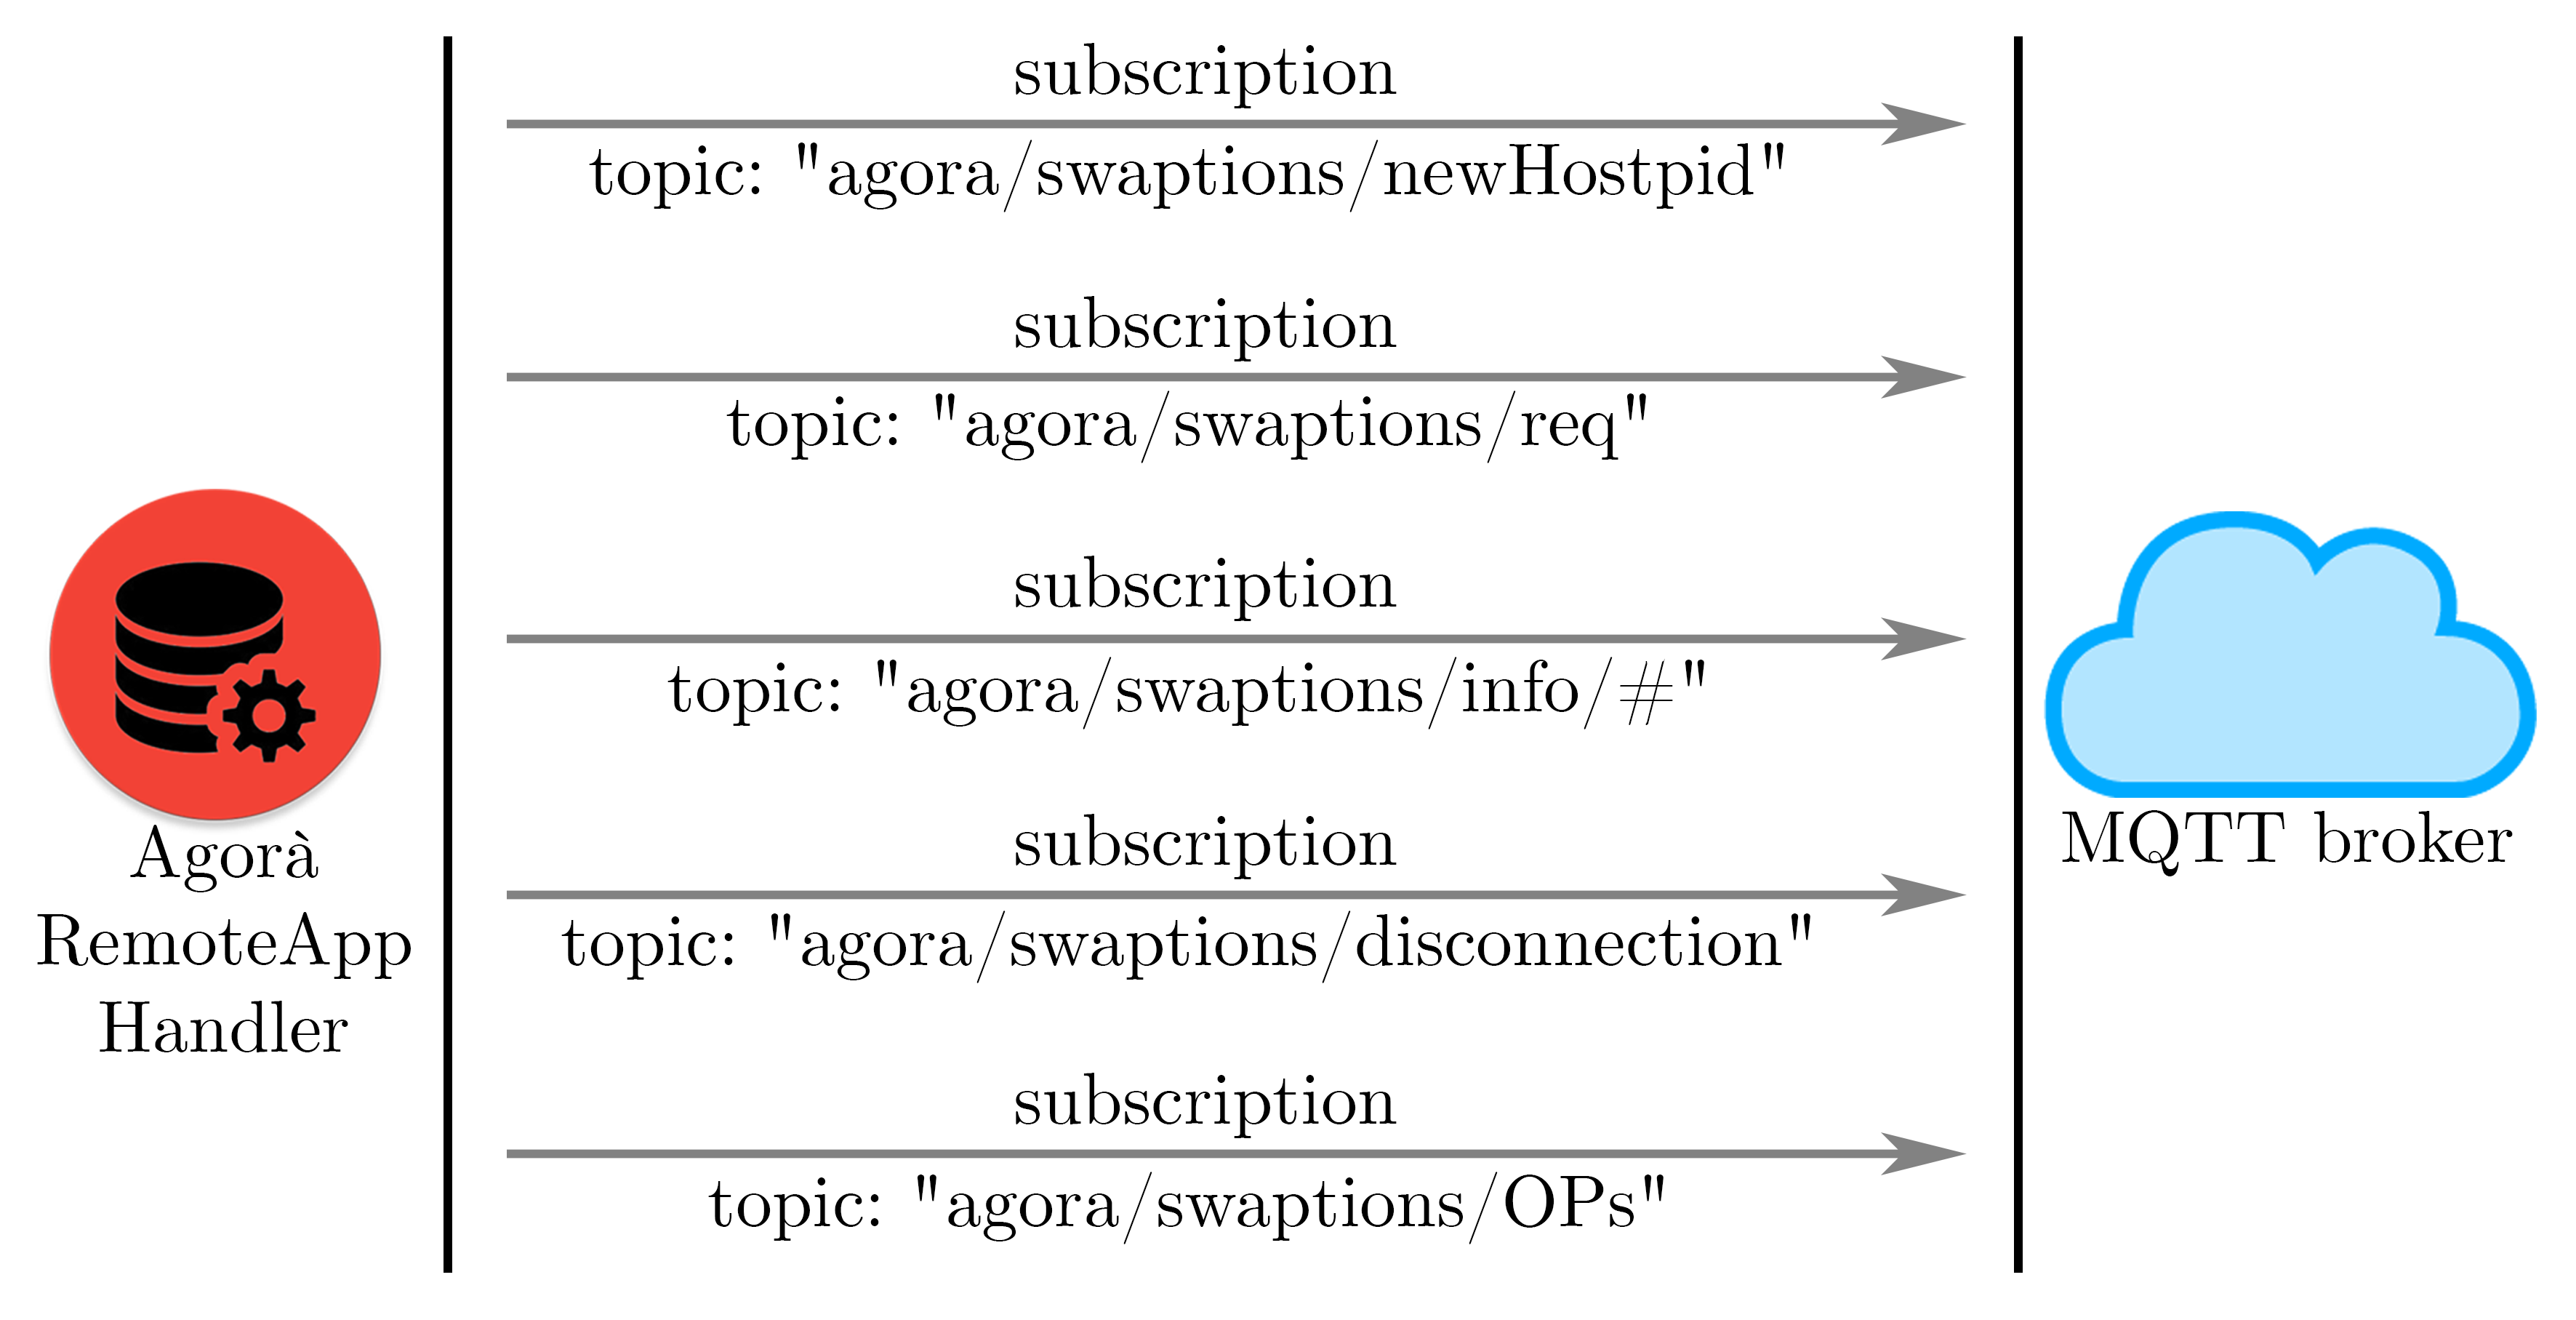
\includegraphics[width = \textwidth]{handler_subs}
    \caption{server\_handler MQTT subscriptions example}
    
\end{figure}


\subsubsection{Known application}\label{knownApp}

When the server\_listener is informed that a new node has started running an application but there is already a ser\-ver\_han\-dler that is managing that program, it publishes on topic "tesiCris/\textit{[appName]}/newHostpid" the new machine hostname plus PID, so that the corresponding server\_handler can add the node to the pool of machines that are running the application it is supervising:

\begin{figure}[H]

    \centering
    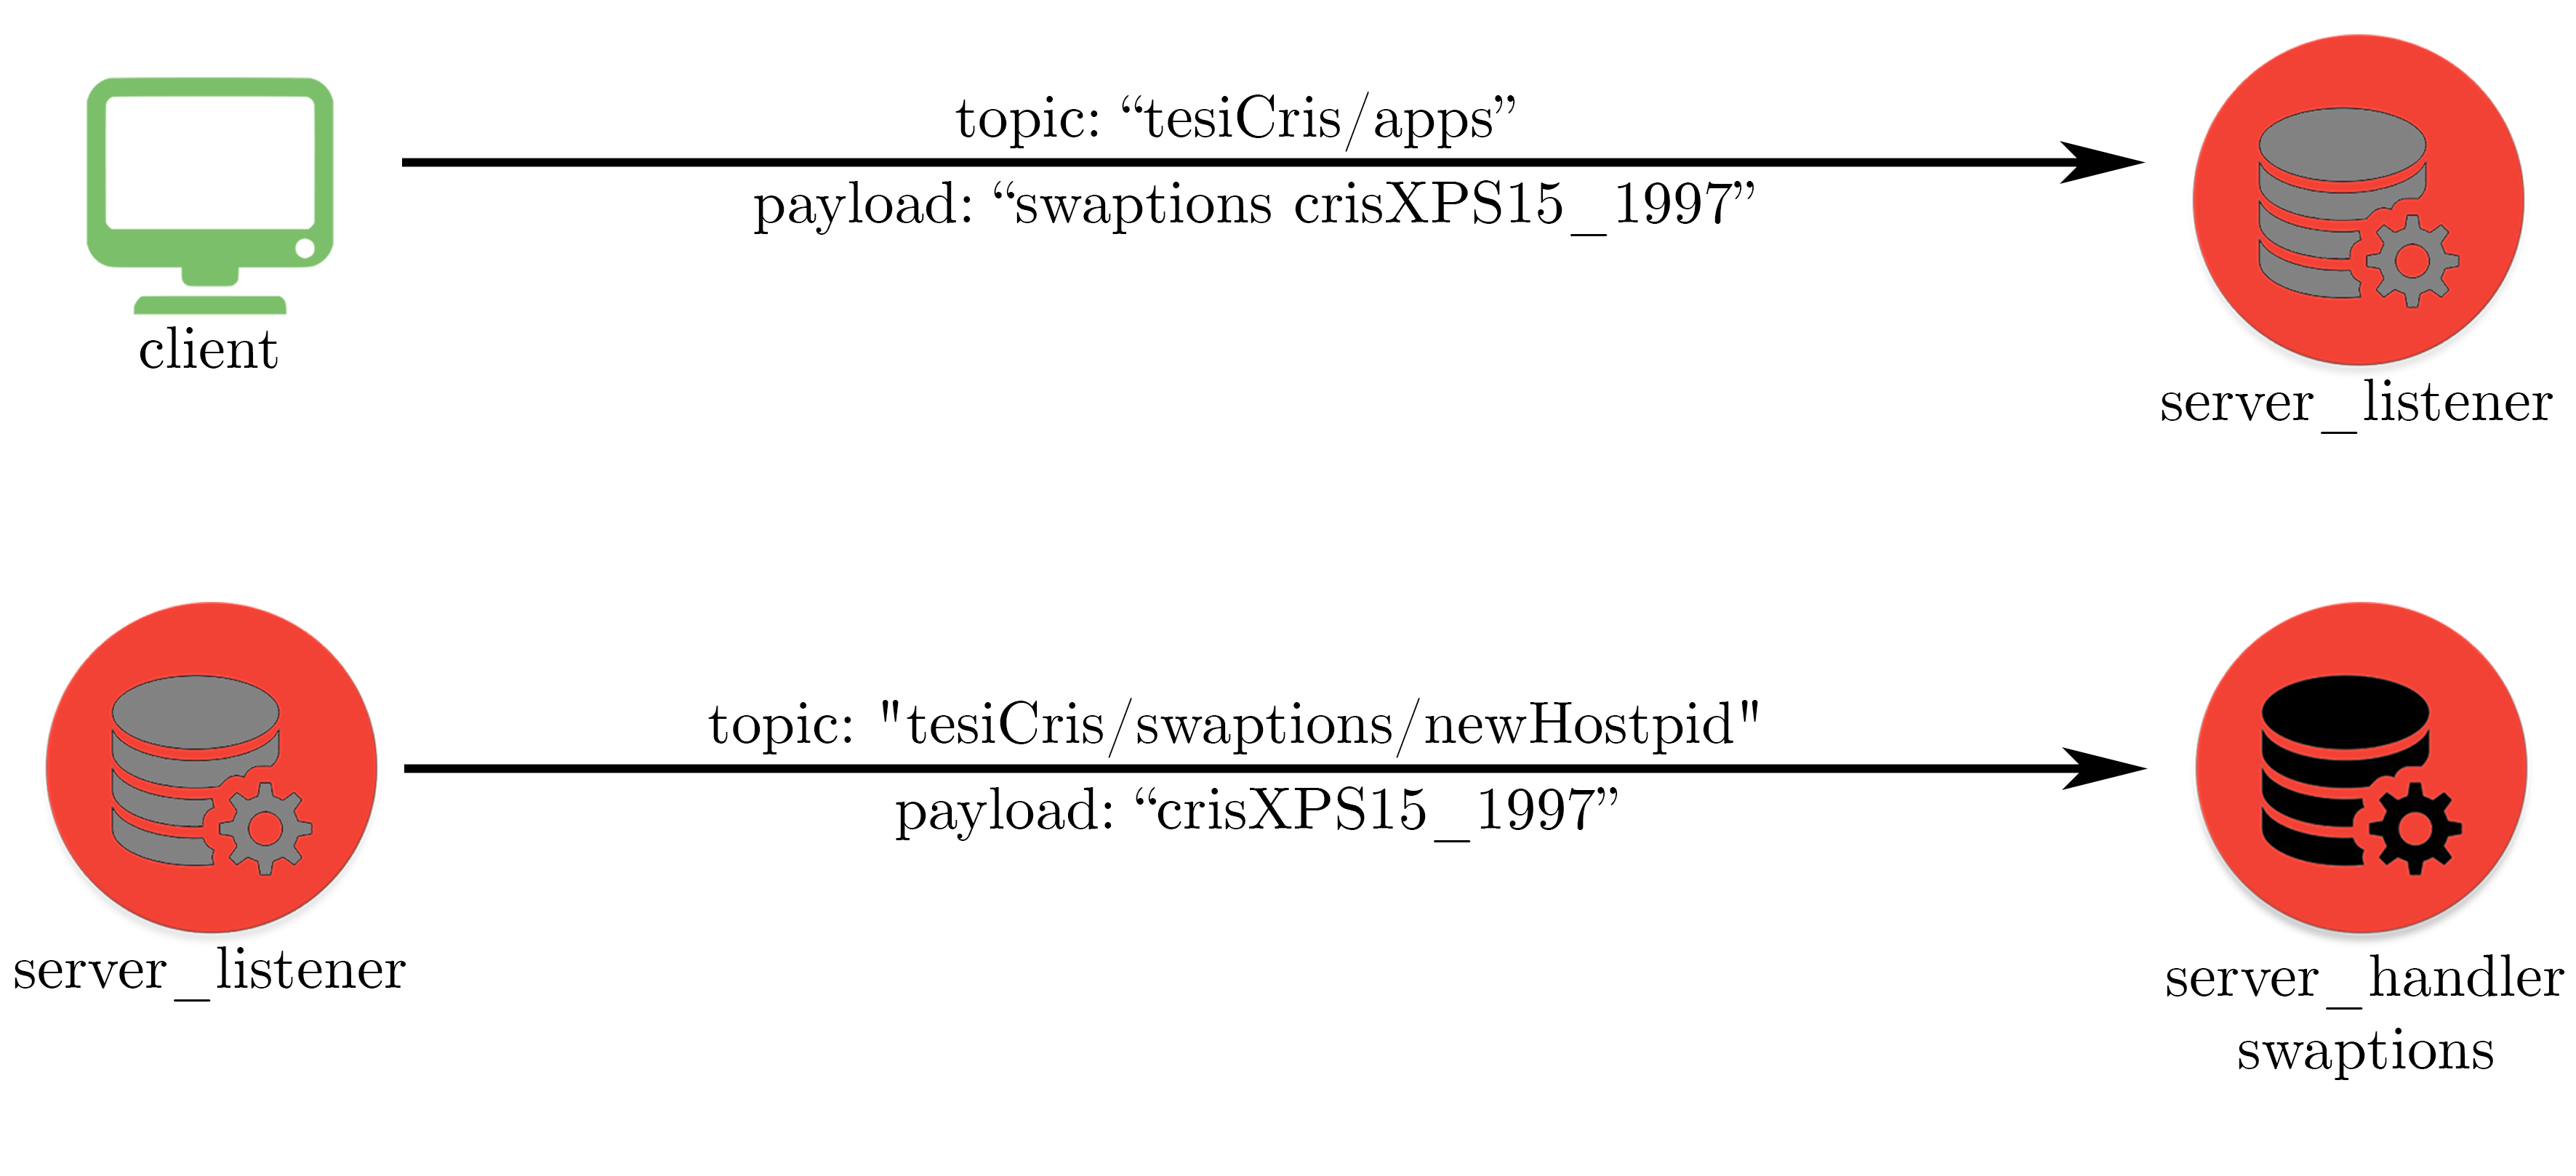
\includegraphics[width = \textwidth]{new_known}
    \caption{New known application arrival example; client ID is sent by the server\_listener to the corresponding server\_handler}
    
\end{figure}





\subsection{Client request}\label{clientReq}

At each predetermined time interval, clients make a request to their application server\_handler, publishing their hostname plus PID on topic "tesiCris/\textit{[appName]}/req":

\begin{figure}[H]

    \centering
    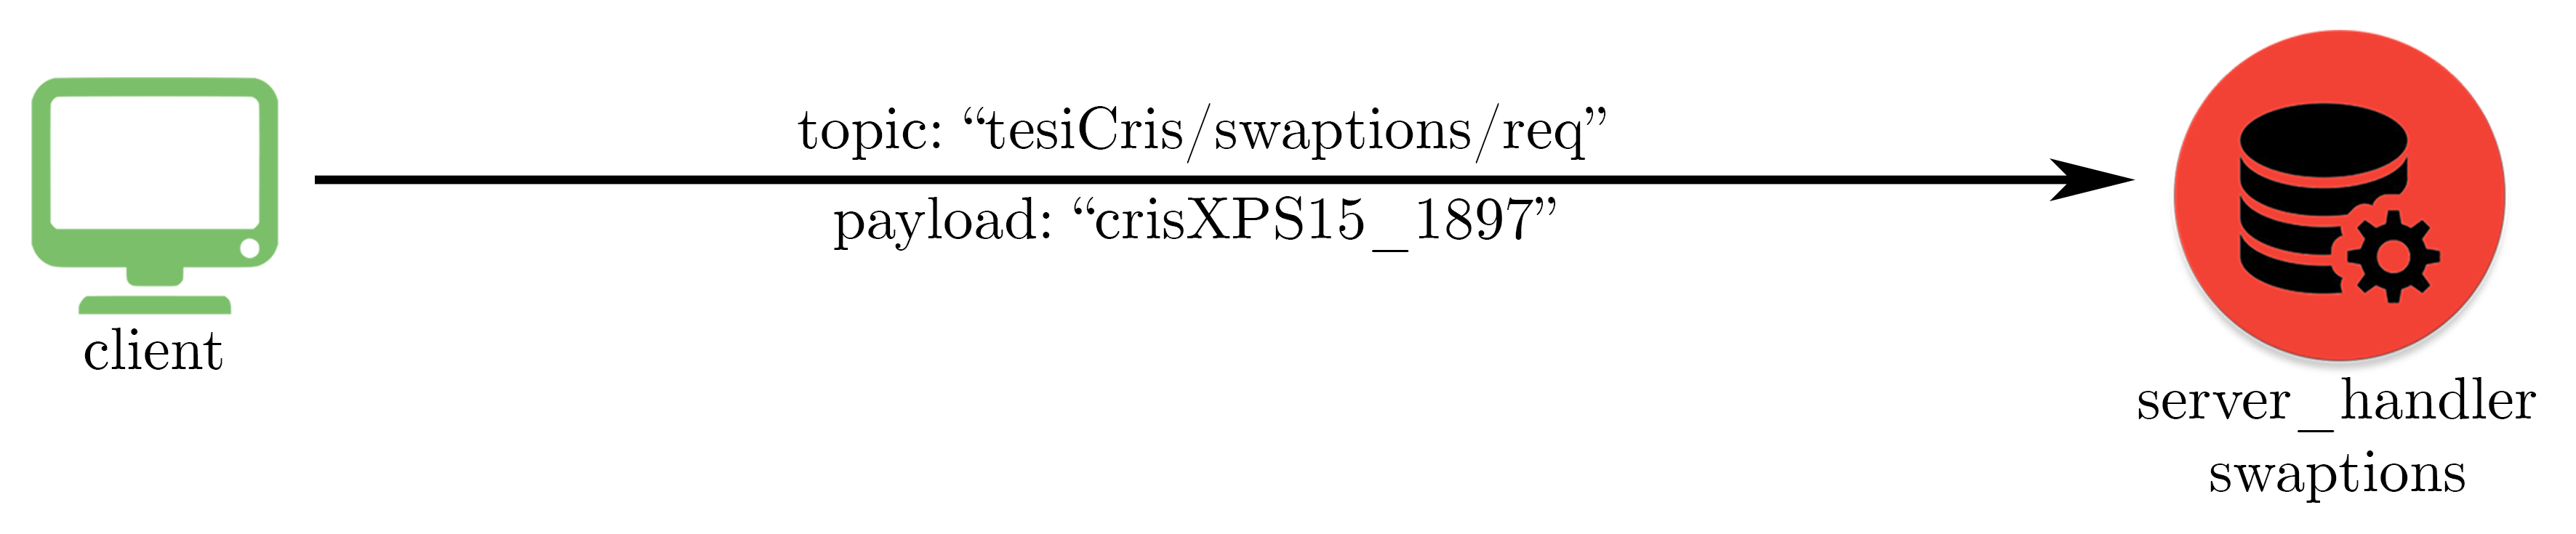
\includegraphics[width = \textwidth]{req}
    \caption{Client request example}
    
\end{figure}

This kind of publication is repeated until the node receives the predicted complete Operating Point list; server\_handler replies to these requests according to its internal state, that can be one of the following:

\begin{enumerate}

    \item \textit{unknown};

    \item \textit{receivingInfo};

    \item \textit{buildingDoE};

    \item \textit{DSE};

    \item \textit{buildingTheModel};

    \item \textit{autotuning}.

\end{enumerate}


\subsubsection{server\_handler \textit{unknown} internal state}\label{req_info}

The server\_handler doesn't know anything about the application it is managing, except its name; it asks to clients all the available information, making a publication with payload "info" on topic "tesiCris/\textit{[appName]}":

\begin{figure}[H]

    \centering
    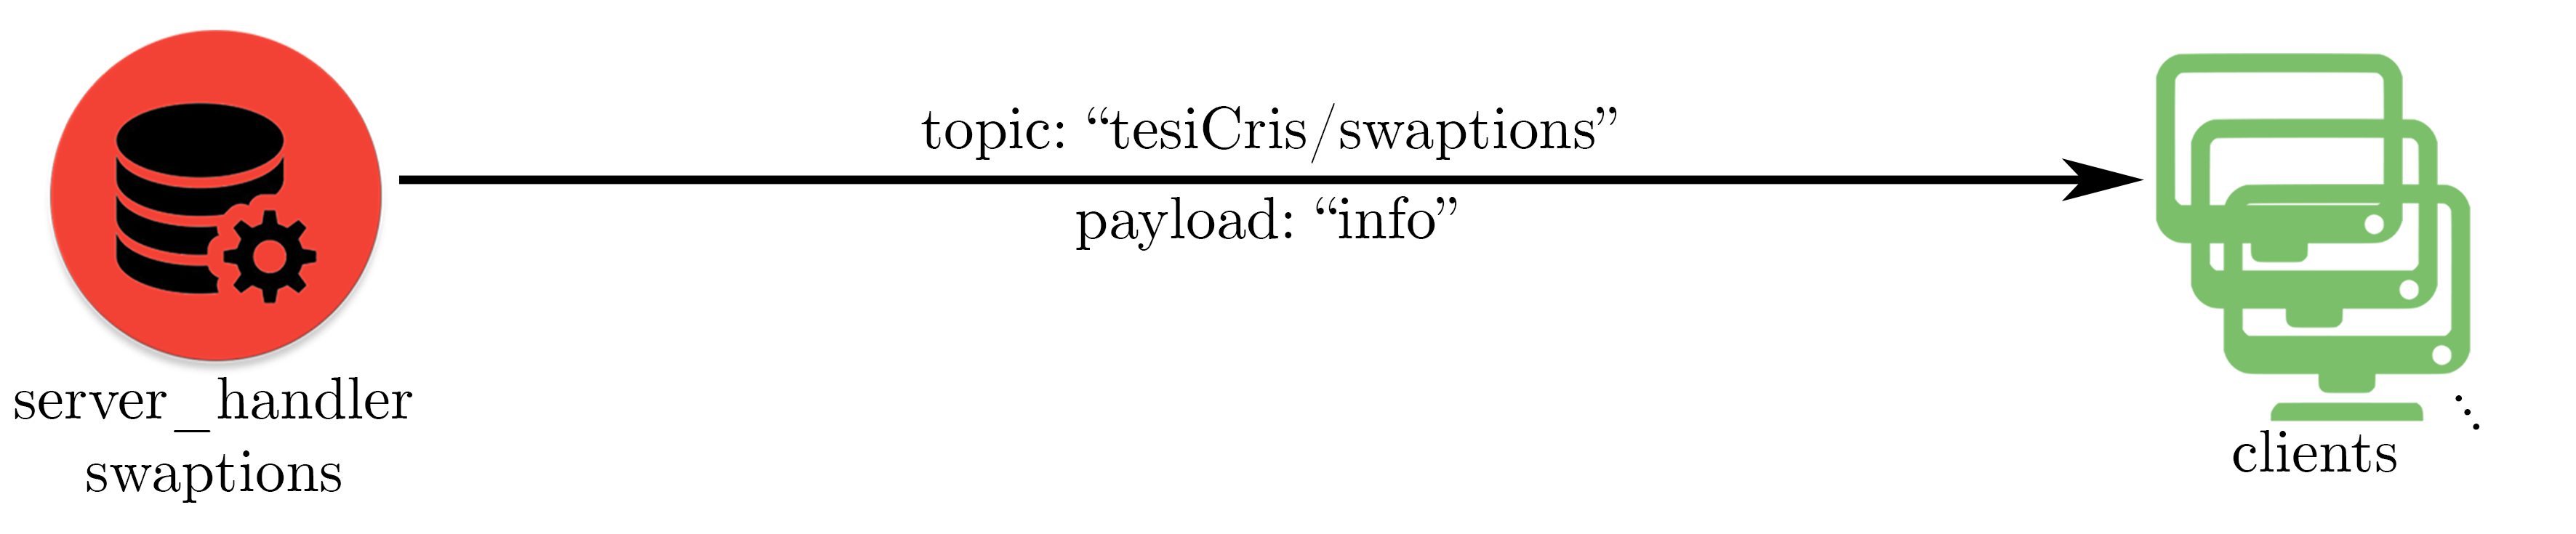
\includegraphics[width = \textwidth]{info_req}
    \caption{Application information request by \textit{AgoràRemoteAppHandler} example}
    
\end{figure}


\subsubsection{server\_handler \textit{receivingInfo} internal state}

The server\_handler is receiving application information, so in this case it discards all possible requests made by clients.


\subsubsection{server\_handler \textit{buildingDoE} internal state}

The server\_handler, according to the received Design of Experiments type (see \ref{client_info}), is building the set of configurations that will be distributed to clients during Design Space Exploration phase; also in this case it discards all possible clients requests.


\subsubsection{server\_handler \textit{DSE} internal state}\label{dse_conf}

The server\_handler has computed DoE configurations, so it is driving Design Space Exploration phase; it picks up the first element on top of the available configurations list and it sends, in lexicographic order, the associated software knobs values on topic "tesiCris\slash{}\textit{[appName]}\slash{}\textit{[hostname]\_[PID]}\slash{}conf", relative to the client that made the request; the configuration just sent is reinserted at the end of the mentioned list:

\begin{figure}[H]

    \centering
    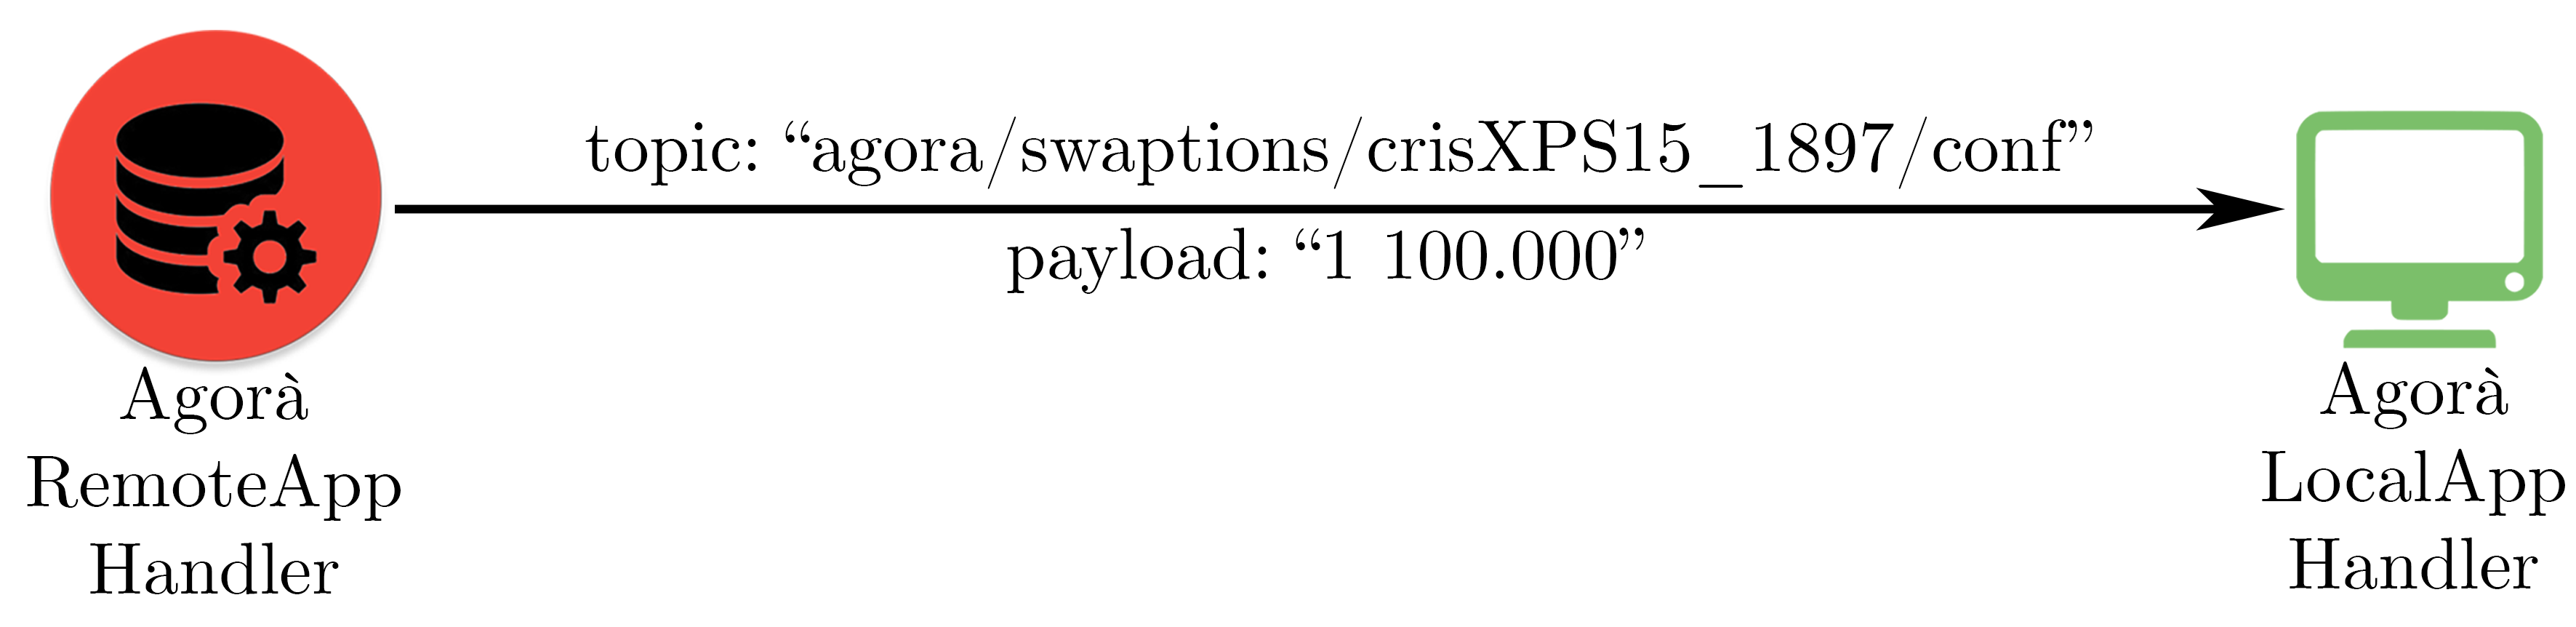
\includegraphics[width = \textwidth]{conf}
    \caption{Configuration dispatch by \textit{AgoràRemoteAppHandler} example}
    \label{fig:conf}
    
\end{figure}

As shown in figure \ref{fig:conf}, client receives a configuration with $num\_threads = 1$ and $num\_trials = 100.000$; the next computation will be done with these parameters values.


\subsubsection{server\_handler \textit{buildingTheModel} internal state}\label{DoEModelSend}

The server\_handler module has gathered all the needed OPs related to DoE configurations and it is computing the complete Operating Points list through Machine Learning techniques; from the gathered Operating Points, a partial model is built, assembling to every DoE configuration the mean of metrics values, taken from the related OPs; this partial model in sent to the client that made the request: every publication is done on topic "tesiCris/\textit{[appName]}/\textit{[hostname]\_[PID]}/model" with payload equal to the computed OP, with format "\textit{[configuration] [metrics values]}"; both configurations and metrics values follow lexicographic order; finally, the server\_handler makes a final publication on the same topic with payload "DoEModelDone":

\begin{figure}[H]

    \centering
    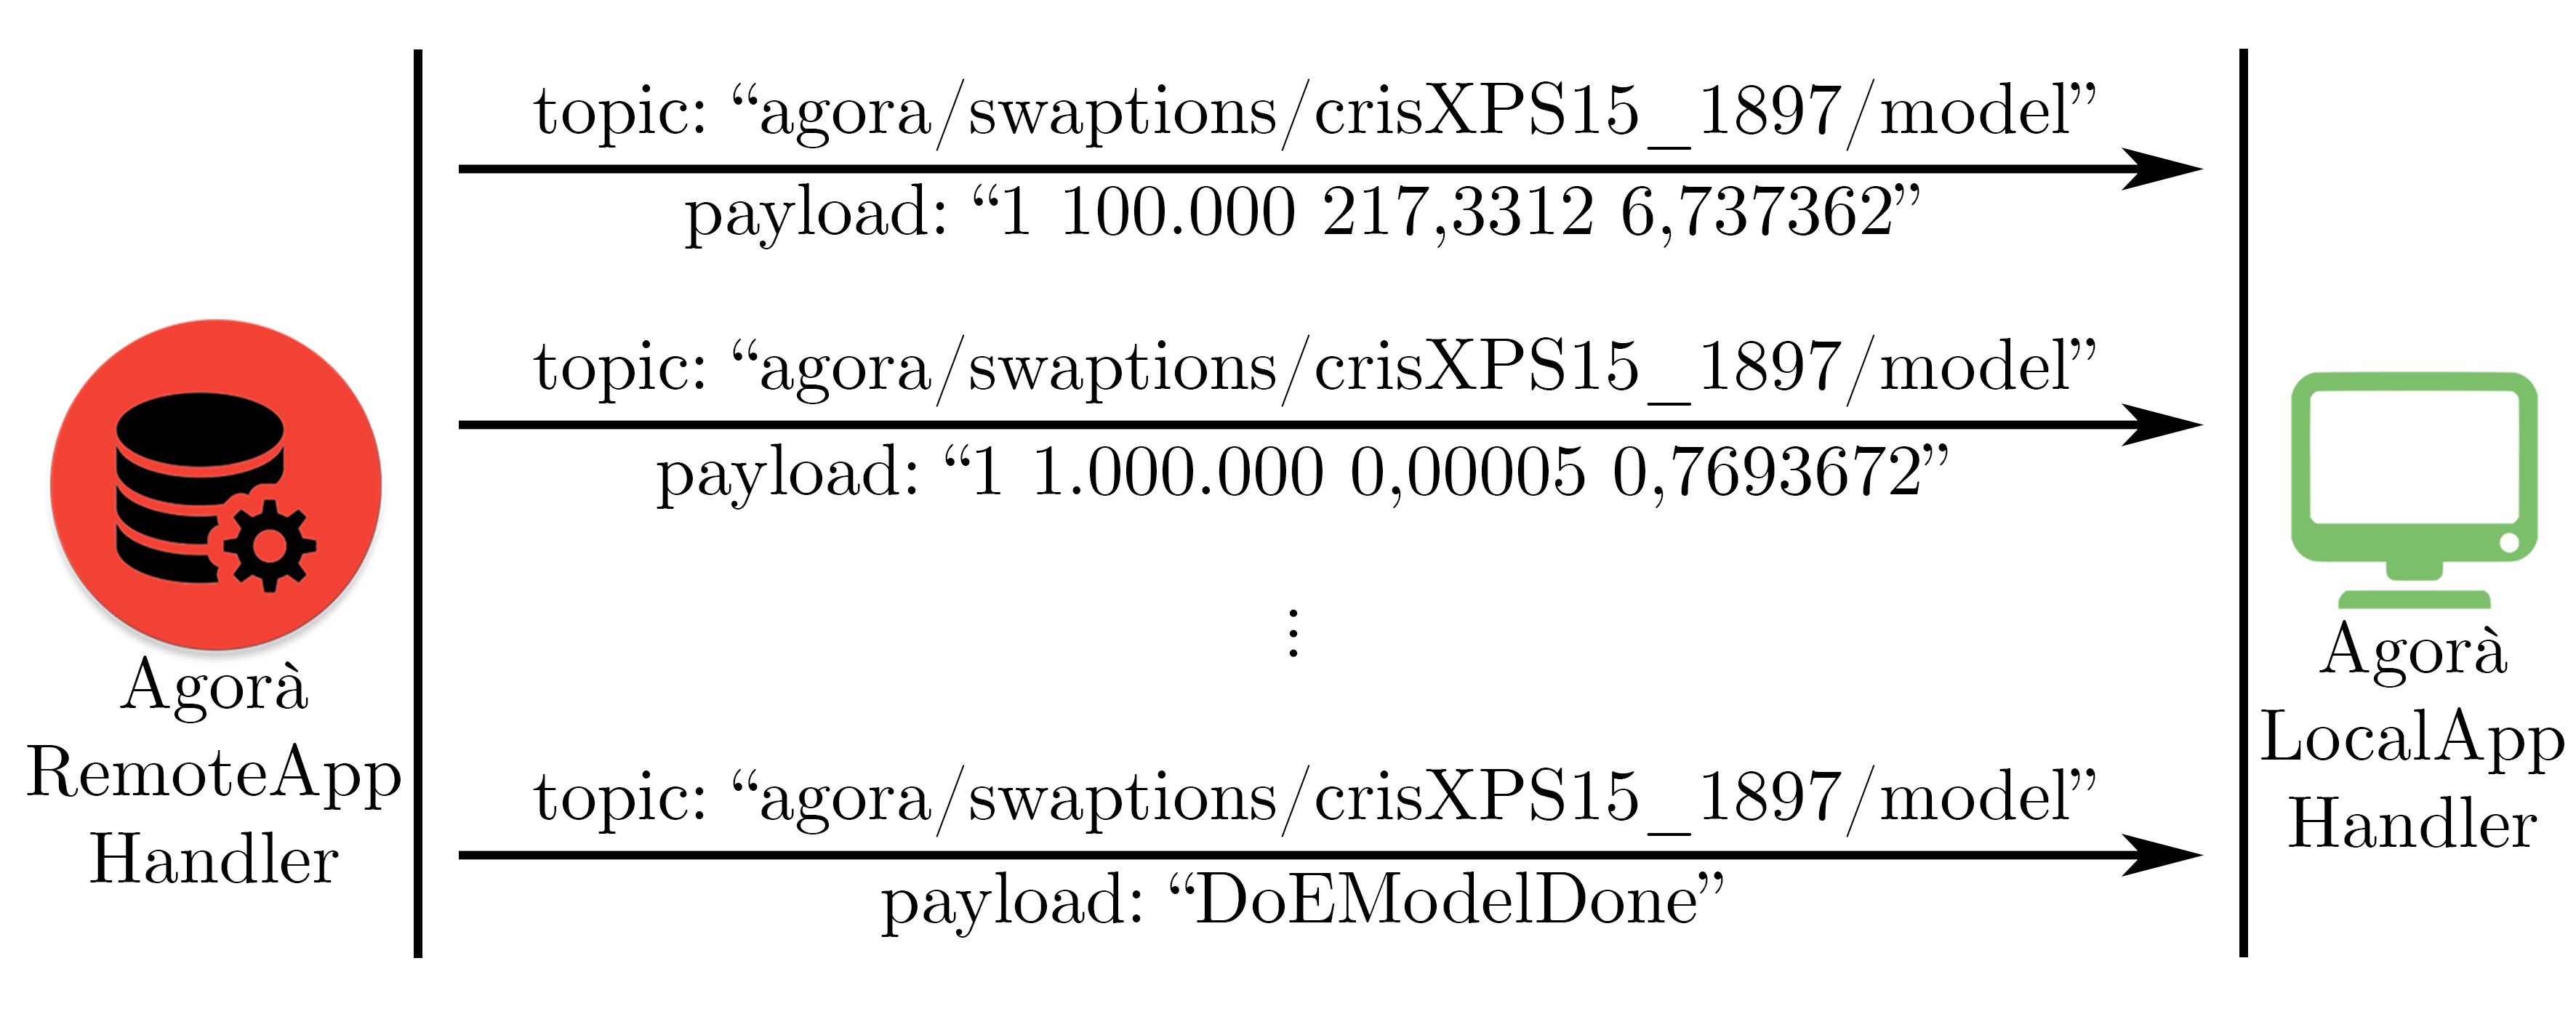
\includegraphics[width = \textwidth]{doe_model}
    \caption{Partial model dispatch by \textit{AgoràRemoteAppHandler} example}
    \label{fig:doe_model}
    
\end{figure}

Taking figure \ref{fig:doe_model} as reference, the first sent OP has parameters\linebreak $num\_threads = 1$ and $num\_trials = 100.000$, with metrics $avg\_error = 217,3312$ and $avg\_throughput = 6,737362$; the client module sets up mARGOt autotuner with this OP list, so the application is executed with the best Operating Point that fulfils current goals and requirements.

\subsubsection{server\_handler \textit{autotuning} internal state}\label{modelSend}

The server\_handler owns the complete OP list, obtained through the Generalized Linear Regression interface by Apache Spark\textsuperscript{TM} MLlib library; similarly to the previous case (\ref{DoEModelSend}), every Operating Point is sent to the client on topic "tesiCris\slash{}\textit{[app\-Name]}\slash{}\textit{[host\-name]\_[PID]}\slash{}model" with format "\textit{[configuration] [metrics values]}", respecting lexicographic order for both parameters and metrics values; the final publication has payload "modelDone":

\begin{figure}[H]

    \centering
    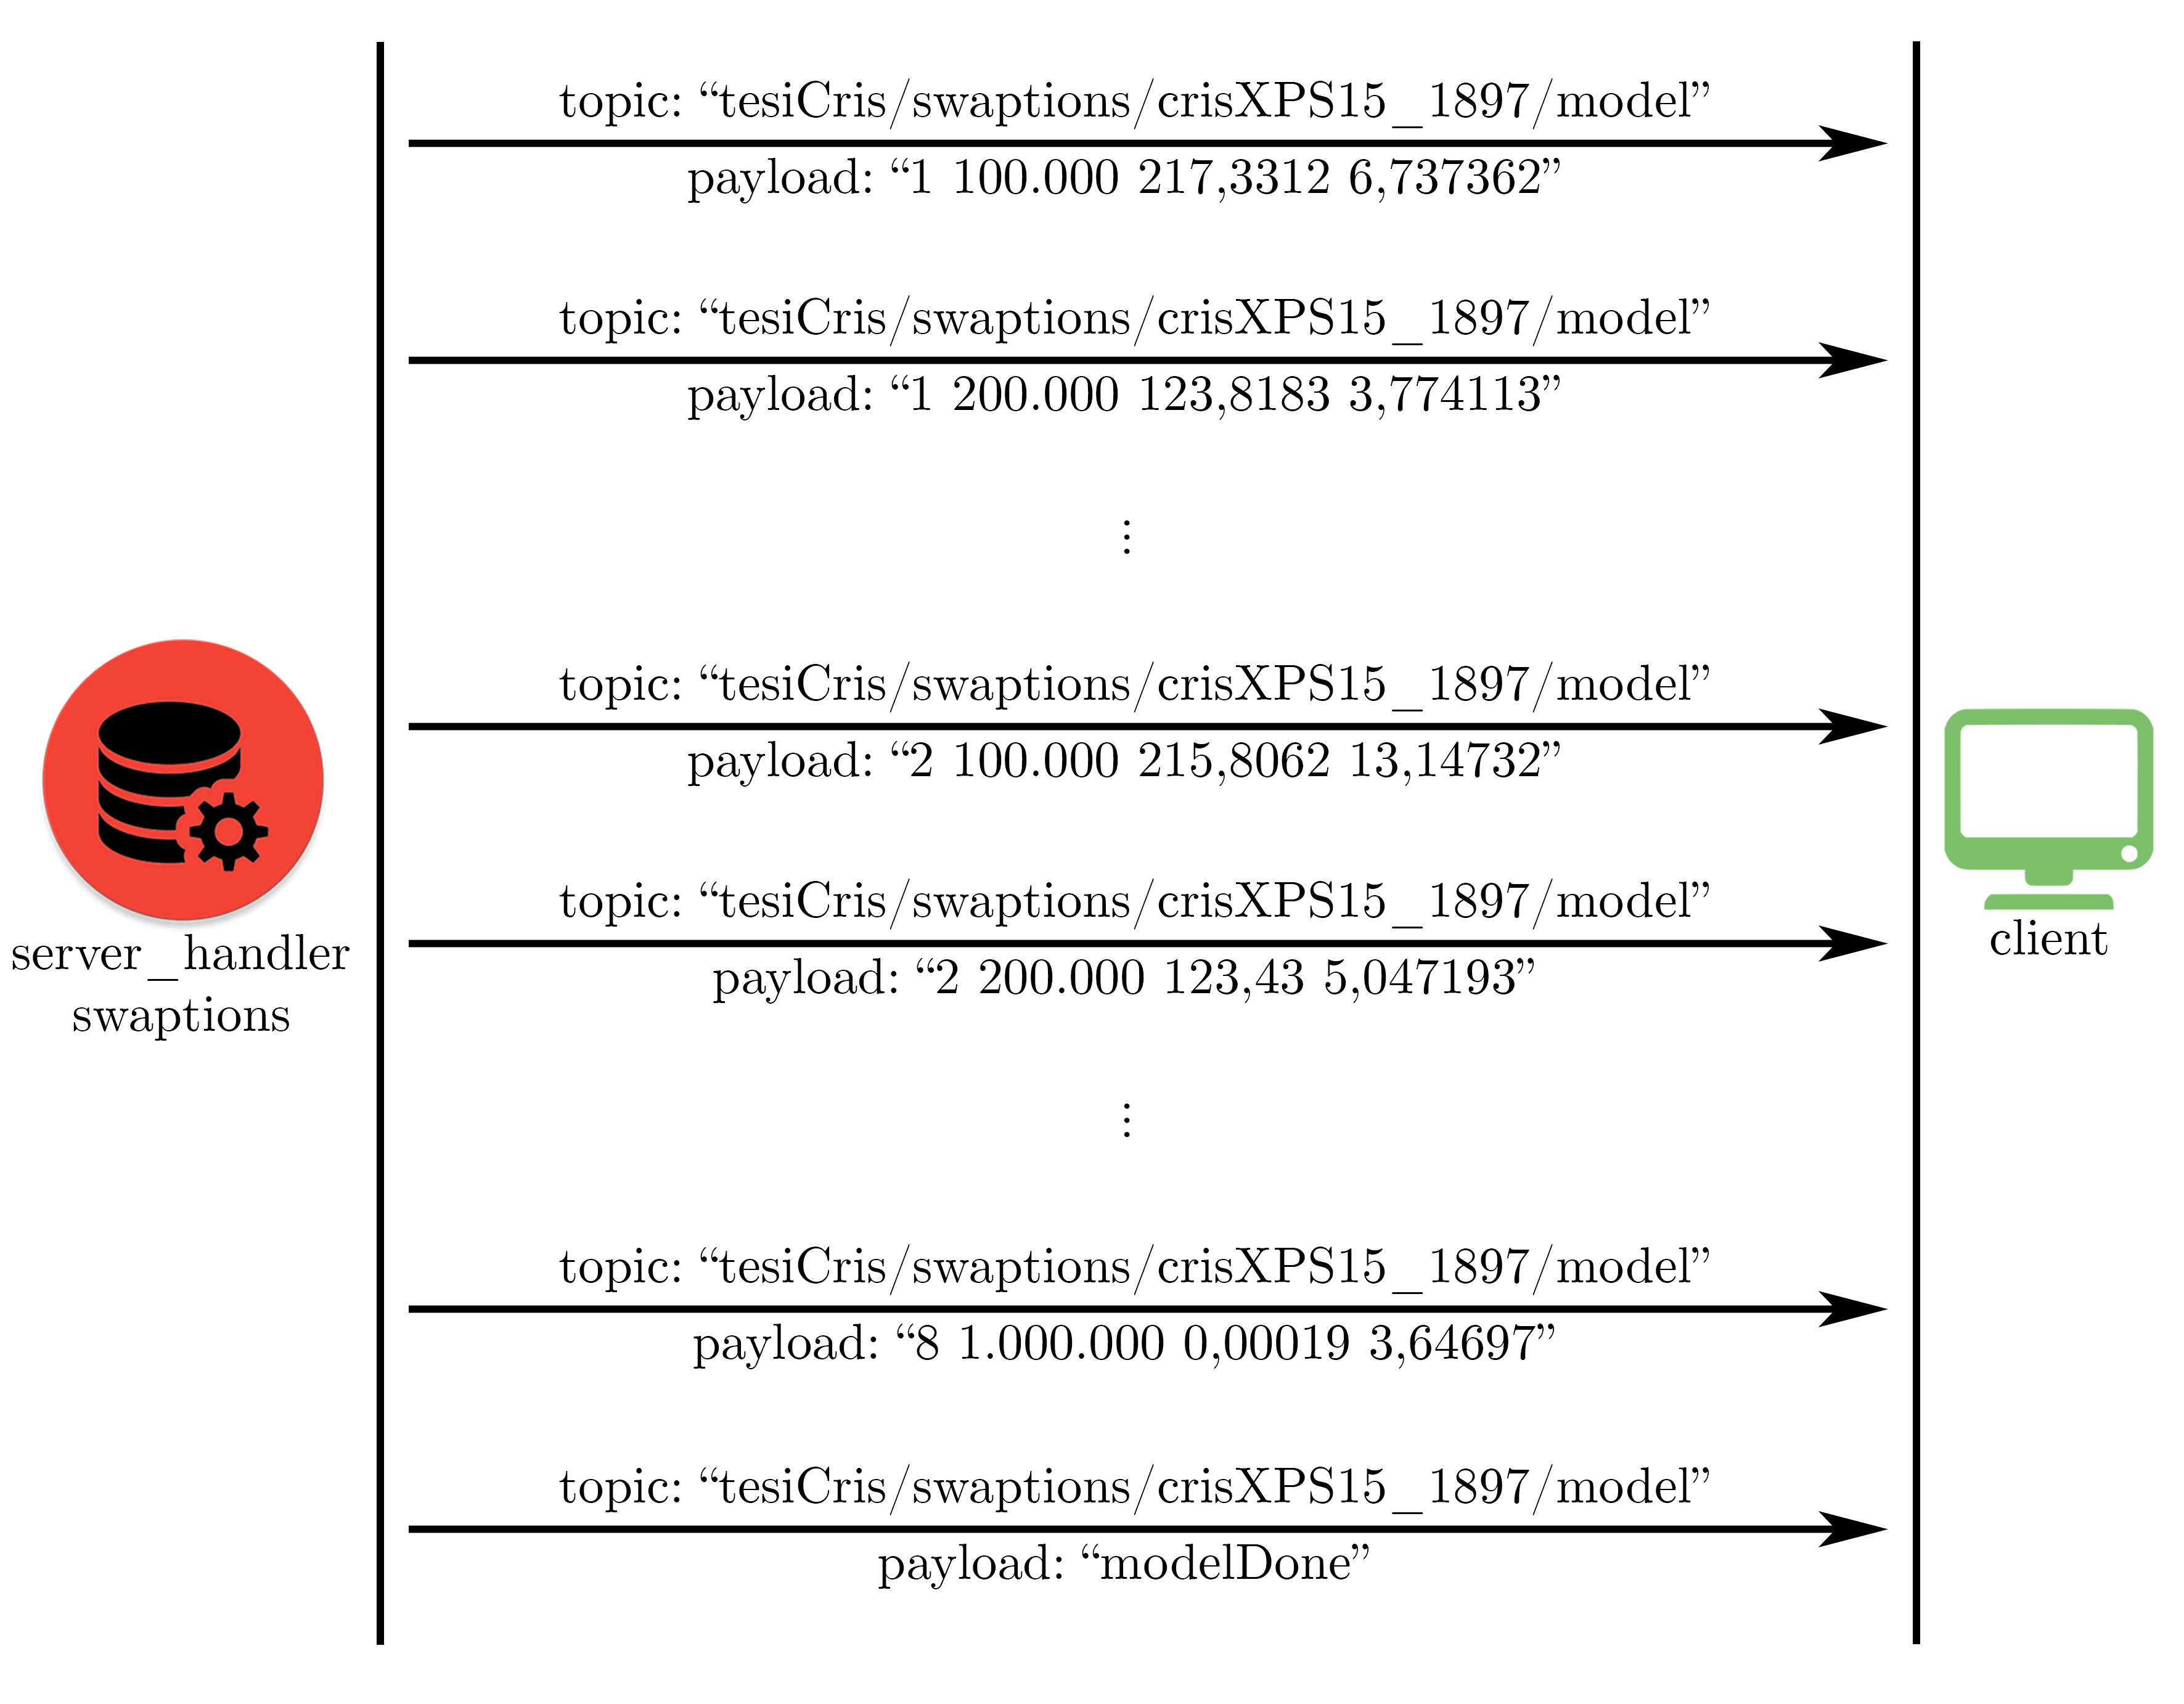
\includegraphics[width = \textwidth]{model}
    \caption{Complete model dispatch by \textit{AgoràRemoteApplicationHandler} example}
    \label{fig:model}
    
\end{figure}

In swaptions application, variable num\_threads can assume 8 different values, while variable num\_trials 10 ones, so the complete model is composed by all the 80 OPs; after mARGOt autotuner has received all the predictions, it can set application knobs according to current objectives.

From this point on, client stops making requests to the ser\-ver\_han\-dler module.





\subsection{Client application information dispatch}\label{client_info}

It has been shown that, if a server\_handler receives a request from a node but its internal state is unknown, it requests application information (see \ref{req_info}); the server\_handler saves both the identifier of the first client that replies and all data it receives; other possible replies from other clients are discarded.

Mandatory information that cilent modules have to send is:

\begin{enumerate}

    \item metrics under examination: the keyword is \textit{metric}, followed by metric name; there is a publication for each metric; publications have to be in lexicographic order with respect to metrics name;
    
    e.g. payload: "metric avg\_throughput"
    
    \item application parameters: the keyword is \textit{param}, followed by parameter name, the way in which it is transmitted and the corresponding values; there is a publication for each parameter; also in this case, publications must follow lexicographic order with respect to parameters name; tesiCris makes available two ways to send values:
    
    \begin{enumerate}
    
        \item by list: the keyword is \textit{enum} and, in this case, all possible values are listed;
        
        \item by extreme values and step: the keyword is \textit{range} and, in this case, minimum value, maximum value and step are sent; the ser\-ver\_han\-dler, from this information, computes all possible parameter values.
    
    \end{enumerate}
    
    e.g. payload: "param num\_threads enum 1 2 3 4 5 6 7 8"
    
    e.g. payload: "param num\_trials range 100.000 1.000.000 100.000"

\end{enumerate}

There are some optional information that clients can send to the ser\-ver\_handler:

\begin{enumerate}

    \item number of required repetitions for each Operating Point: the keyword is \textit{numReps}, followed by a number; this value represents the number of Operating Points that the server\_handler has to gather for each Design of Experiments configuration, during Design Space Exploration phase;
    
    e.g. payload: "numReps 5"
    
    \item Design of Experiments type: the keyword is \textit{DoE}, followed by the term that indicates the kind of Design of Experiments that has to be used; it can be:
    
    \begin{enumerate}
    
        \item \textit{fcccd}: it corresponds to the Face Centered Central Composite DoE with one Center Point;
        
        \item \textit{ff2l}: it corresponds to the 2-Level Full-Factorial DoE;
        
        \item \textit{pbd}: it corresponds to the Plackett-Burman DoE;
        
        \item \textit{lhd}: it corresponds to the Latin-Hypercube DoE; in this case, there is another optional information that can be sent to the server\_handler: the number of configurations that have to be produced, with the word \textit{lhdSamples} followed by the desired value; if this information is not sent, the number of random configurations is equal to the number of application parameters;
        
        \item \textit{fcccdExtra}: it corresponds to the Face Centered Central Composite DoE with one Center Point plus the addition of other configurations through the Latin-Hypercube DoE; as in the previous case, the optional keyword \textit{lhdSamples} is used to express the number of extra configurations, otherwise they are equal to the number of parameters;
        
        \item \textit{fullFact}: it corresponds to the Full-Factorial DoE.
    
    \end{enumerate}
    
    Design of Experiments concepts are explained in chapter \ref{doe}.
    
    e.g. payload: "DoE fcccdExtra"
    
    e.g. payload: "lhdSamples 6"
    
    \item Response Surface Modeling technique: the keyword is \textit{RSM}, followed by the term that indicates the Machine Learning technique that has to be used in order to predict the complete OP list; tesiCris has implemented two versions of the Apache Spark\textsuperscript{TM} Generalized Linear Regression RSM, explained in detail in \ref{regrTransforms}:
    
    \begin{enumerate}
    
        \item the first, that uses parameters values transformations, with associated word \textit{sparkGenLinRegrTransforms};
        
        \item the second, that uses parameters polynomial expansion of second order, with associated word \textit{sparkGenLinRegr2ndPolyExp}
    
    \end{enumerate}
    
    e.g. payload: "RSM sparkGenLinRegr2ndPolyExp"
    
    \item parameters values transformations for the first implemented version of Apache Spark\textsuperscript{TM} Generalized Linear Regression RSM: the keyword is \textit{paramsTransforms}, followed by the involved metric name and the terms that indicate the kind of parameters transformations, the family distribution and the link function.
    
    Transformations must follow the same order of parameters information dispatch; they can be:
    
    \begin{enumerate}
    
        \item \textit{inv}: in this case, to the corresponding parameter values in the OPs, the inverse function is applied;
        
        \item \textit{ln}: in this case, to the corresponding parameter values in the OPs, the natural logarithmic function is applied;
        
        \item \textit{sqrt}: in this case, to the corresponding parameter values in the OPs, the square root function is applied;
        
        \item \textit{id}: in this case, the corresponding parameter values in the OPs are not transformed.
    
    \end{enumerate}
    
    tesiCris has focused on the prediction of continuous functions with normal distribution: the corresponding family is the Gaussian one, indicated with word \textit{gaussian}.
    
    For the Gaussian family, the link function can be:
    
    \begin{enumerate}
    
        \item \textit{identity};
        
        \item \textit{log};
        
        \item \textit{inverse}.
    
    \end{enumerate}
    
    If this kind of information is available, it must exist for each metric of interest.
    
    e.g. payload: "paramsTransforms avg\_error id sqrt gaussian log"
    
    \item number of application features: the keyword is \textit{numFeats}, followed by the corresponding number; in this case, a minimum number \textit{n} of features values observations can be specified through the keyword \textit{minNumObsFeatsValues}, followed by \textit{n}: only those features values that are observed at least \textit{n} times, during Design Space Exploration phase, contribute to the prediction of the complete OP list; if no features value reaches \textit{n} observations, \textit{n} becomes the number of observations of the most observed features value; if this last information is missing, $n = 1$.
    
    e.g. payload: "numFeats 1"
    
    e.g. payload: "minNumObsFeatsValues 5"

\end{enumerate}

If not specified, the default Design of Experiments type is Face Centered Central Composite DoE with one Center Point, the default number of repetitions for each OP is 1, the default number of program features is 0 and the default RSM technique is the implemented second version of the Apache Spark\textsuperscript{TM} Generalized Linear Regression. If the chosen RSM technique is the GLR first version but there is no information about parameters values transformations, tesiCris tries every possible combination in union with all possible link functions, choosing the best result according to Akaike Information Criterion value and the mean of the sum of coefficient standard errors (see \ref{regrTransforms}).

All the information is sent by clients on topic "tesiCris\slash{}\textit{[appName]}\slash{}info\slash{}\textit{[hostname]\_[PID]}"; a final publication with message "done" specifies to the server\_handler that application information is finished:

\begin{figure}[H]

    \centering
    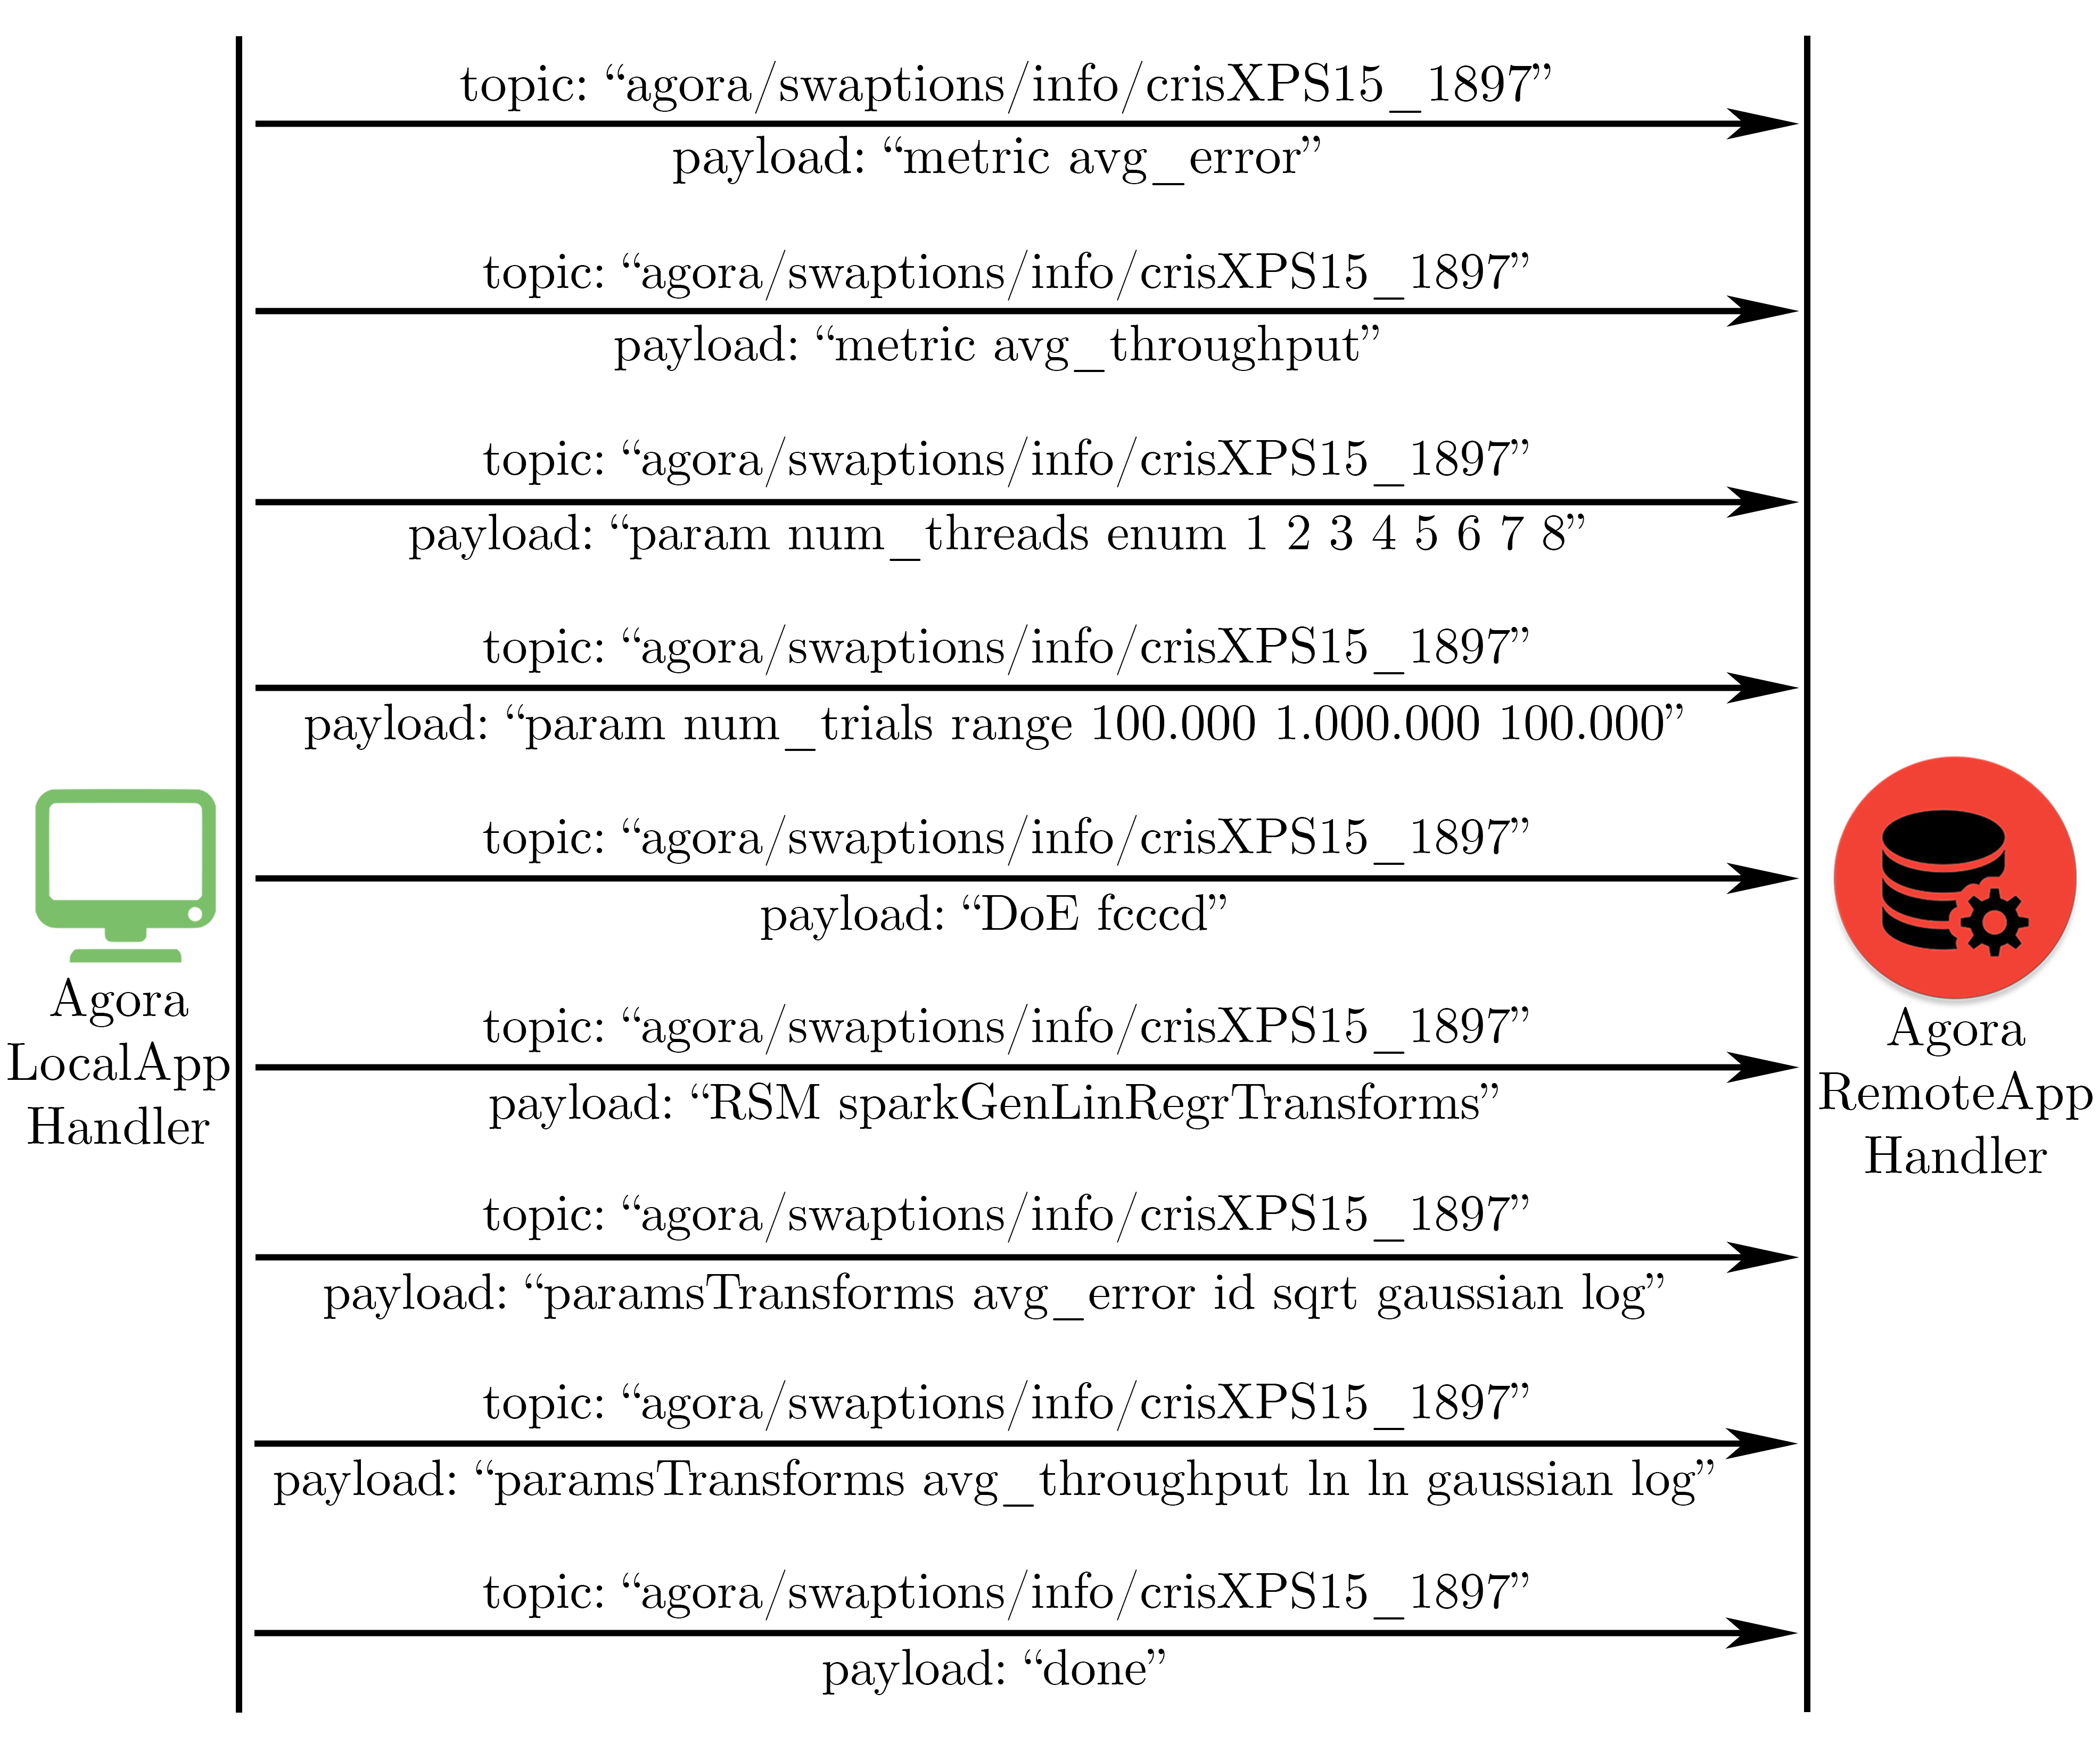
\includegraphics[width = \textwidth]{info_send}
    \caption{Application information dispatch by \textit{AgoràLocalAppHandler} example}
    \label{fig:info_send}
    
\end{figure}

Taking figure \ref{fig:info_send} as reference, the server\_handler pulls out, from topic, \textit{crisXPS15\_1897} and it saves this identifier as the client that is sending program information; this application focuses on two metrics, \textit{avg\_error} and \textit{avg\_throughput}; it has two parameters, \textit{num\_threads} and \textit{num\_trials}; the first is sent with the complete list of values, while the latter is sent with the keyword \textit{range}, specifying its minimum value ($100.000$), its maximum one ($1.000.000$) and the step ($100.000$): the server\_handler computes all values, that are therefore $100.000, 200.000, 300.000, ..., 1.000.000$; the Design of Experiments that has to be used is the Face Centered DoE with one Center Point and the RSM technique is the first implemented version of the Apache Spark\textsuperscript{TM} Generalized Linear Regression; features transformations are also specified so, e.g. for metric \textit{avg\_error}, the first parameter (\textit{num\_threads}) will not be transformed, while the second parameter (\textit{num\_trials}) has to be transformed with the square root function, applying \textit{gaussian} as family distribution and \textit{log} as link function; it can be noticed that there is no information about the number of Operating Points repetitions to gather during DSE phase: in this case the default value is used (one repetition for each OP); finally, there is no payload with keyword \textit{numFeats} either: the application does not have features.

The server\_handler is now ready to compute Design of Experiments configurations; after that, it can start distributing them to the nodes, driving the subsequent Design Space Exploration phase.





\subsection{Client Operating Point dispatch}\label{opSend}

During DSE, clients store the configurations that receive from the ser\-ver\_han\-dler (see \ref{dse_conf}); every time a configuration is sent, if the current one differs from the new one, the client module communicates to mARGOt autotuner new parameters values; software knobs are set up, therefore the next program computation is executed with new parameters values.

After the execution, client module arranges the obtained Operating Point, composed by the set of parameters values and the observed metrics of interest; it publishes on topic "tesiCris/\textit{[appName]}/OPs" a message in the form "\textit{[configuration]}:\textit{[metrics values]}", in which both values lists have to follow lexicographic order with respect to parameters and metrics name:

\begin{figure}[H]

    \centering
    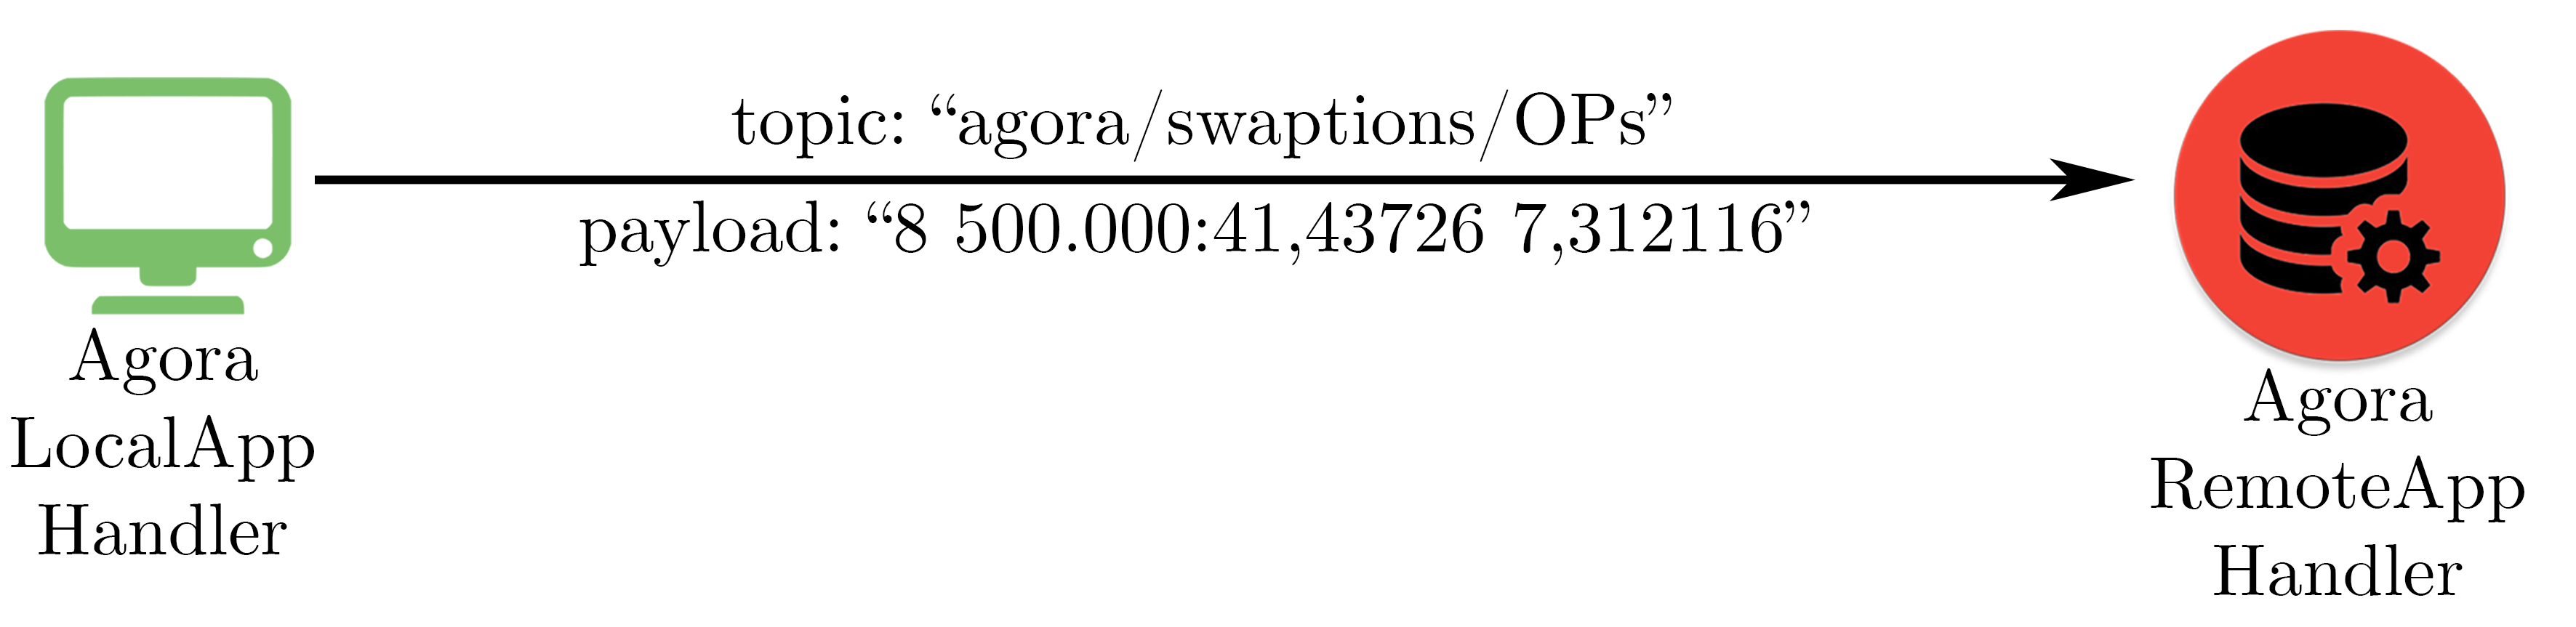
\includegraphics[width = \textwidth]{op}
    \caption{Operating Point dispatch by \textit{AgoràLocalAppHandler} example}
    \label{fig:op}
    
\end{figure}

In the example above, the application has been just executed with\linebreak $num\_threads = 8$ and $num\_trials = 500.000$; monitored metrics values are $avg\_error = 41,43726$ and $avg\_throughput = 7,312116$.

When the server\_handler receives an OP, it decrements the corresponding number of needed Operating Points repetitions: if the updated value is equal to zero, it means that there is no need of other related OPs, so the configuration is moved from the set of available ones to the set of accomplished ones.

The model prediction just starts when the last needed Operating Point repetition for the last available configuration is received from a node.





\subsection{Client disconnection}\label{client_disc}

If a client disconnects for some reason, the server\_handler receives a message on topic "tesiCris\slash{}\textit{[appName]}\slash{}disconnection" with payload "\textit{[hostname]\_[PID]}", relative to the disconnected client; the ser\-ver\_han\-dler removes the node identifier from the list of machines that it is managing:

\begin{figure}[H]

    \centering
    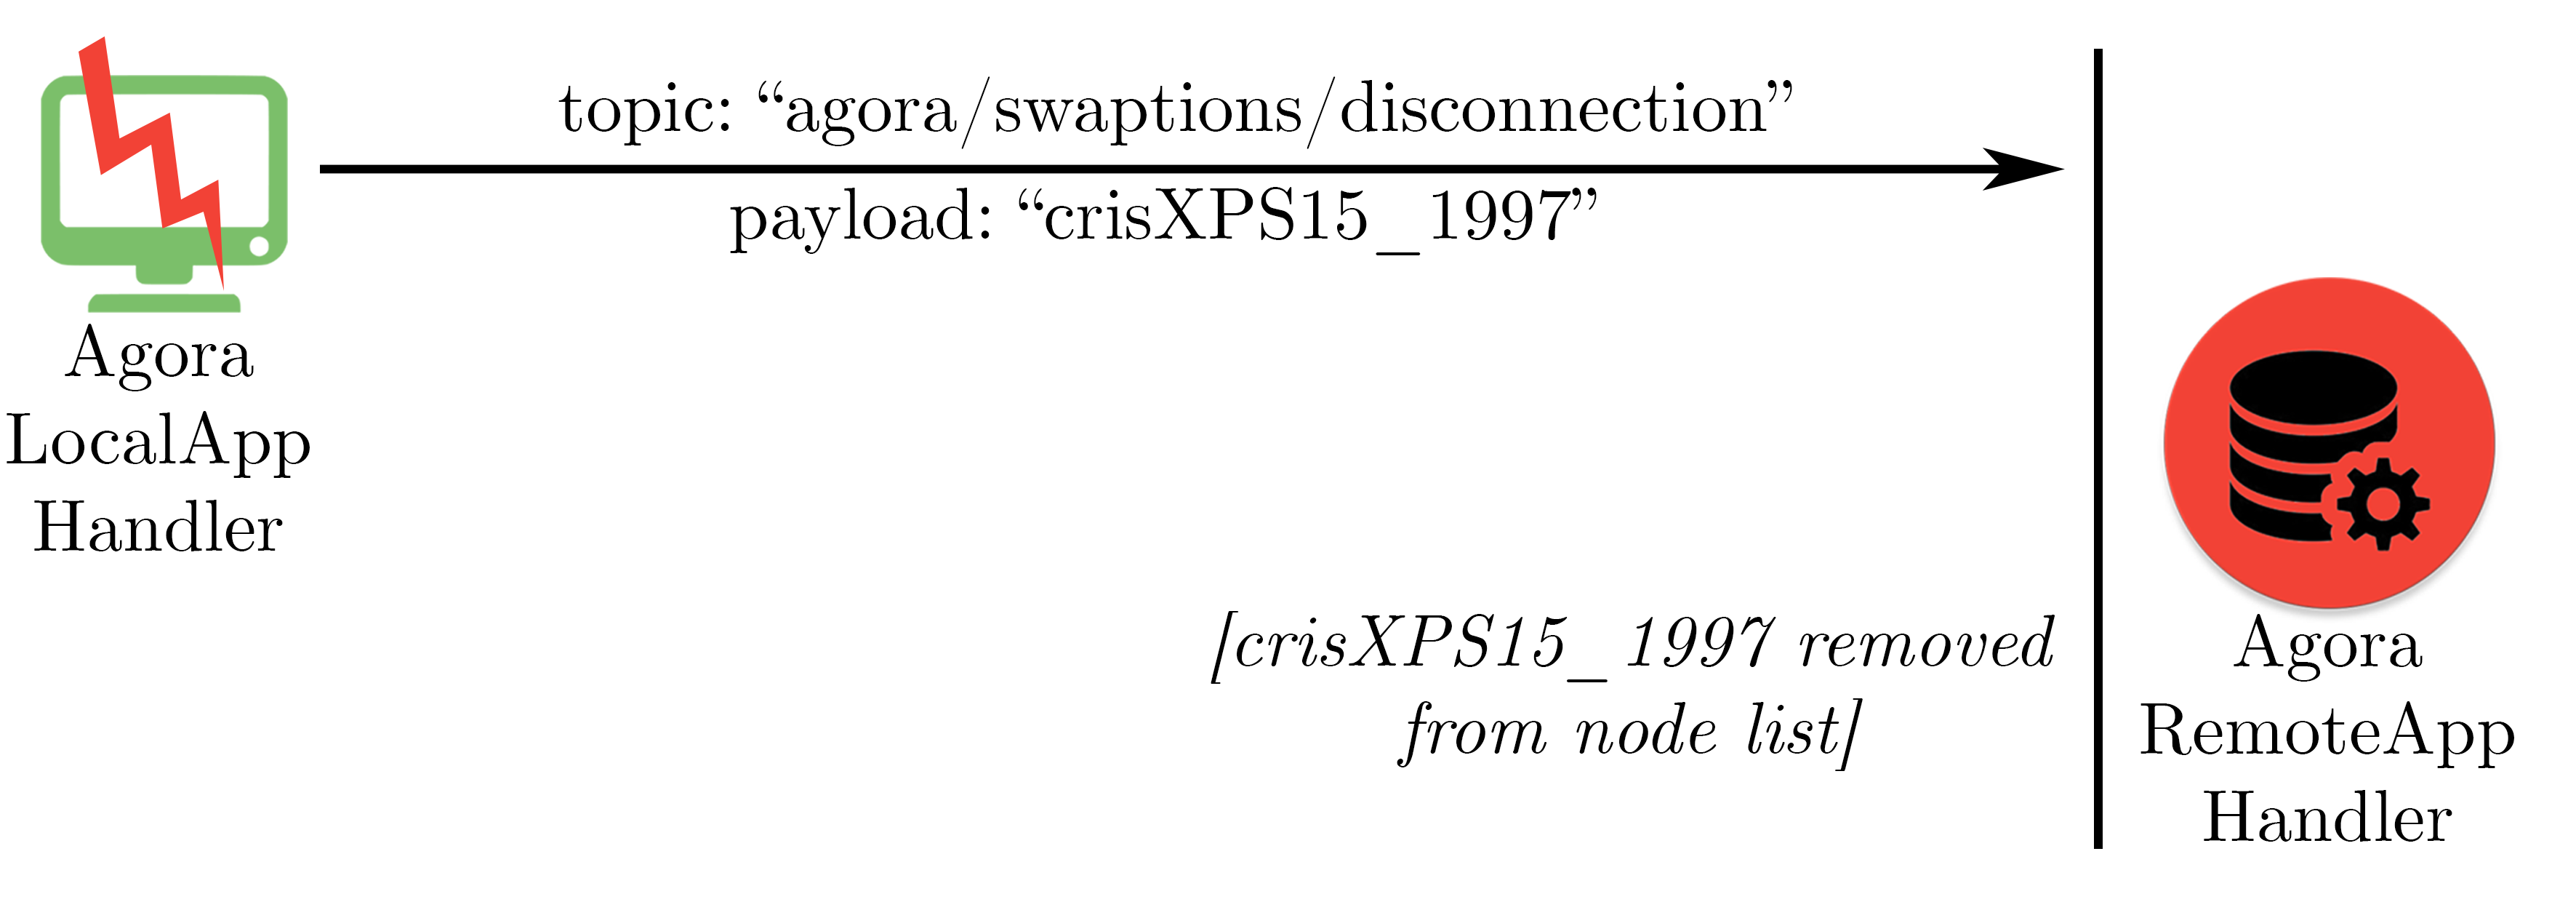
\includegraphics[width = \textwidth]{client_disc}
    \caption{client disconnection example}
    
\end{figure}

Particular attention has to be taken if the disconnected client is the one that, at the beginning, is sending application information (see \ref{client_info}): in this case, the server\_handler has to remove the disconnected machine, it has to reset partial data (received up to that moment) and it asks again all the available application information to remaining connected clients:

\begin{figure}[H]

    \centering
    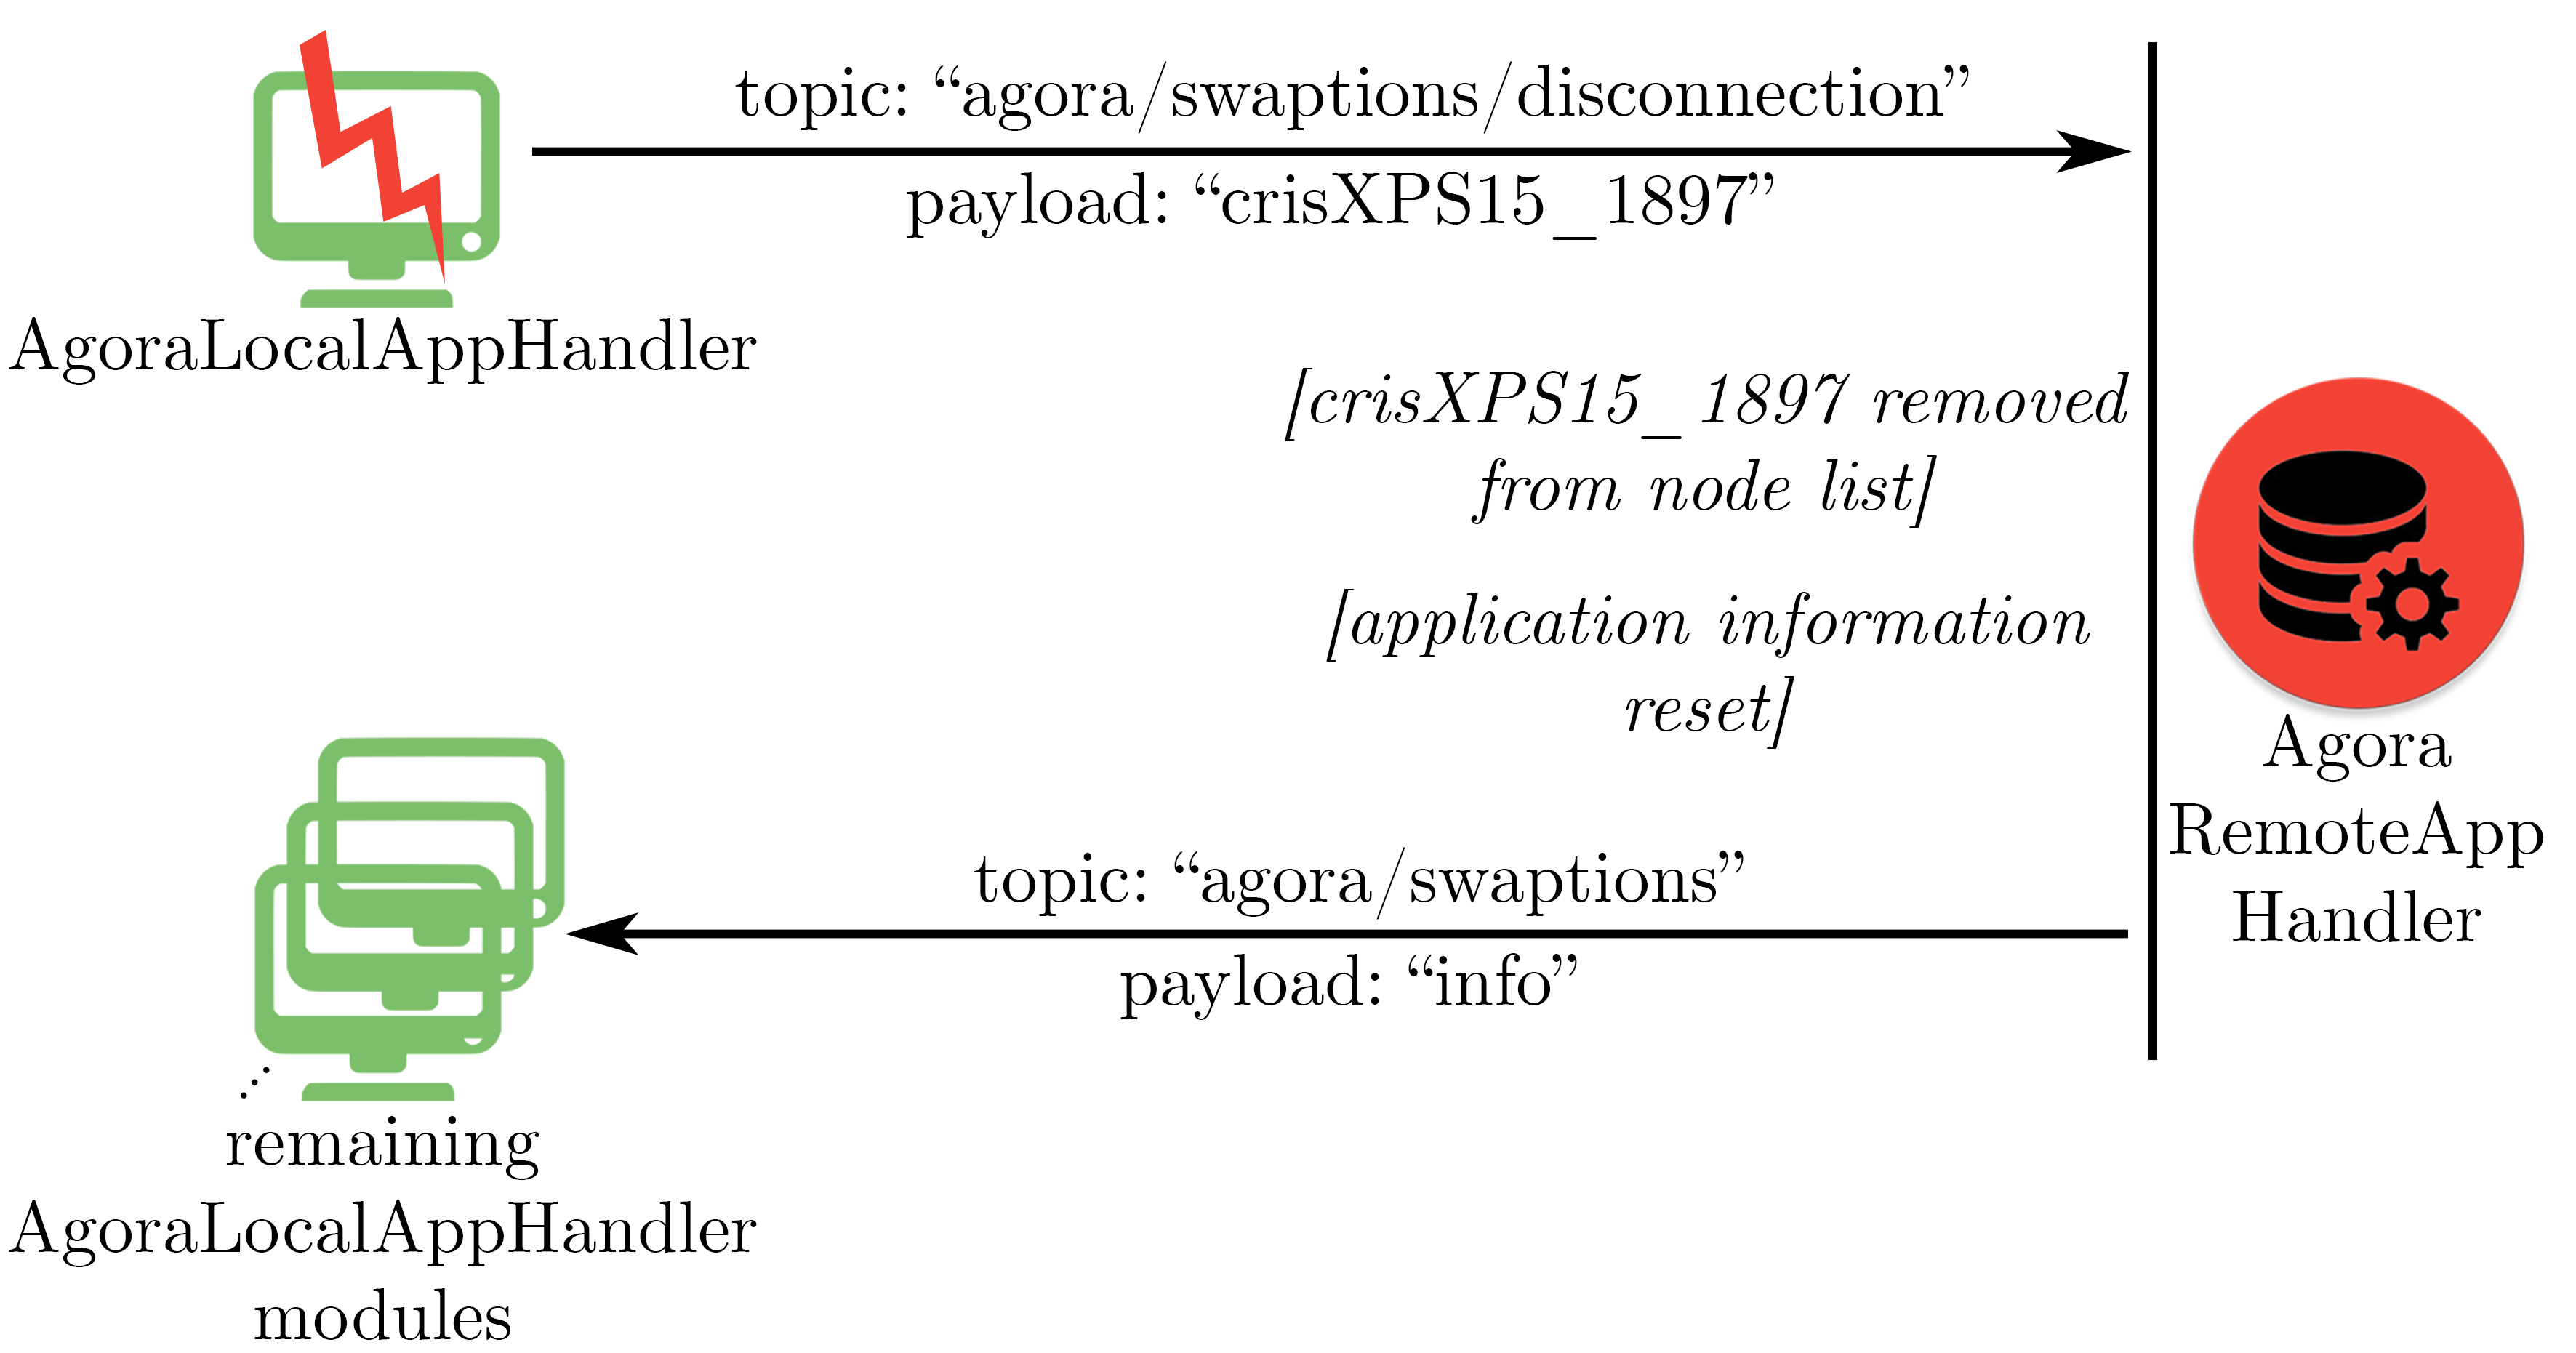
\includegraphics[width = \textwidth]{infoclient_disc}
    \caption{Disconnection of \textit{AgoràLocalAppHandler} that was sending application information example}
    
\end{figure}





\subsection{server\_handler disconnection}\label{handler_disc}

If the server\_handler disconnects, clients receive a message on topic "tesiCris\slash{}\textit{[appName]}" with payload "disconnection":

\begin{figure}[H]

    \centering
    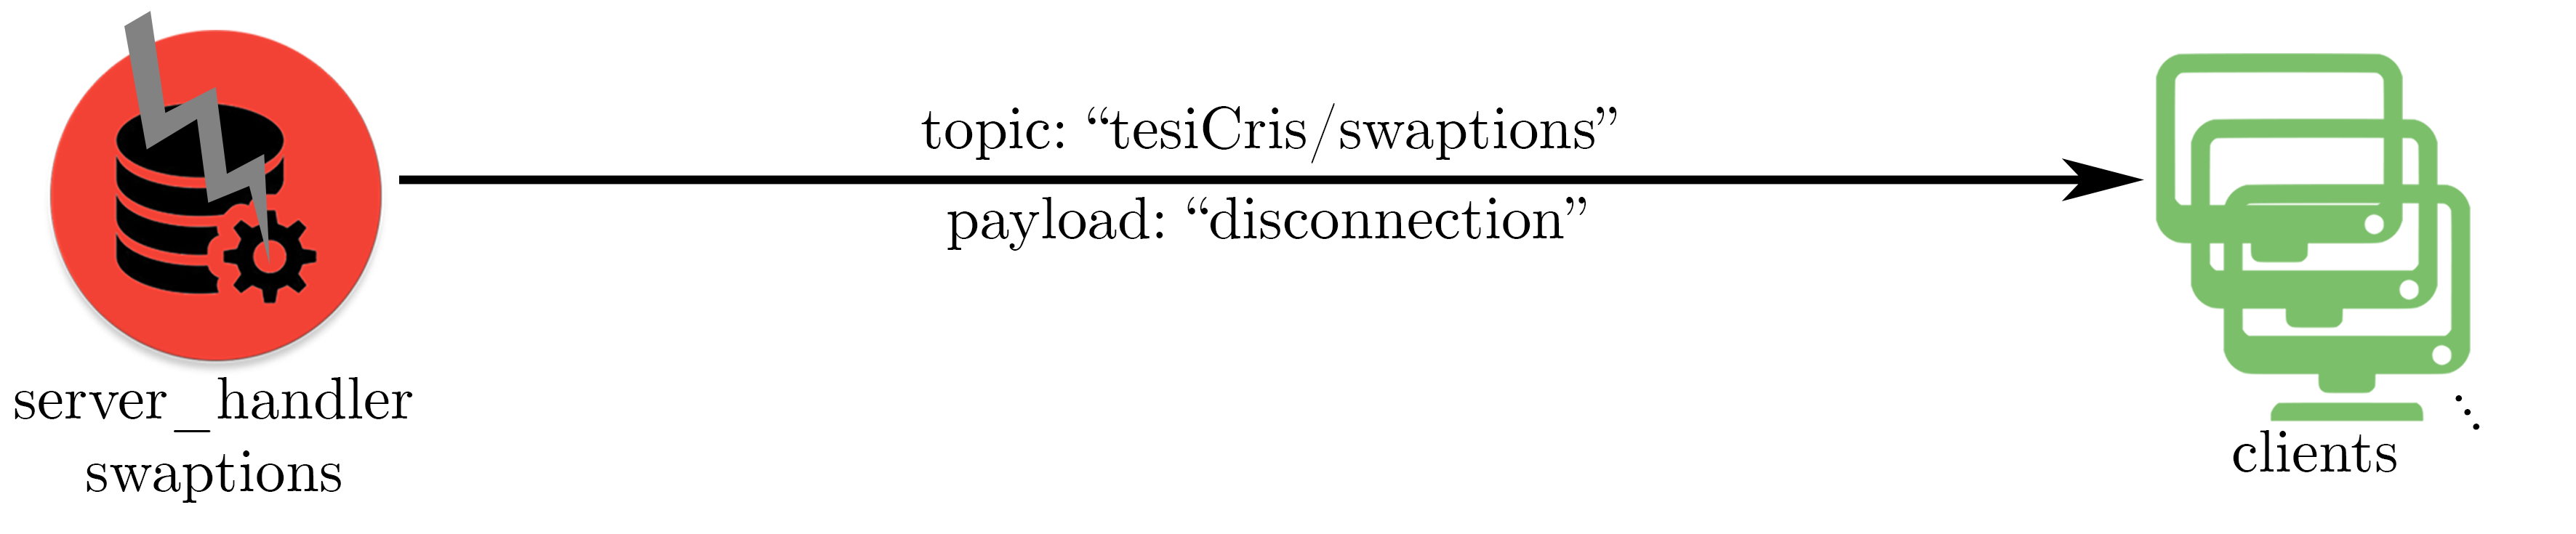
\includegraphics[width = \textwidth]{server_disc}
    \caption{server\_handler disconnection example}
    
\end{figure}

Each client reacts to this event according to its internal state, that can be:

\begin{enumerate}

    \item \textit{defaultStatus};
    
    \item \textit{DSE};
    
    \item \textit{DoEModel};
    
    \item \textit{autotuning}.

\end{enumerate}


\subsubsection{client \textit{defaultStatus} internal state}

When a node starts running, the autotuner sets up application parameters values with a predetermined default configuration; if any Design Space Exploration phase has not been started yet, the server\_handler disconnection doesn't affect application behavior.


\subsubsection{client \textit{DSE} internal state}

The server\_handler is driving Design Space Exploration phase, sending configurations to clients; in this case, the default configuration is restored and the application is executed with the corresponding parameters values:

\begin{figure}[H]

    \centering
    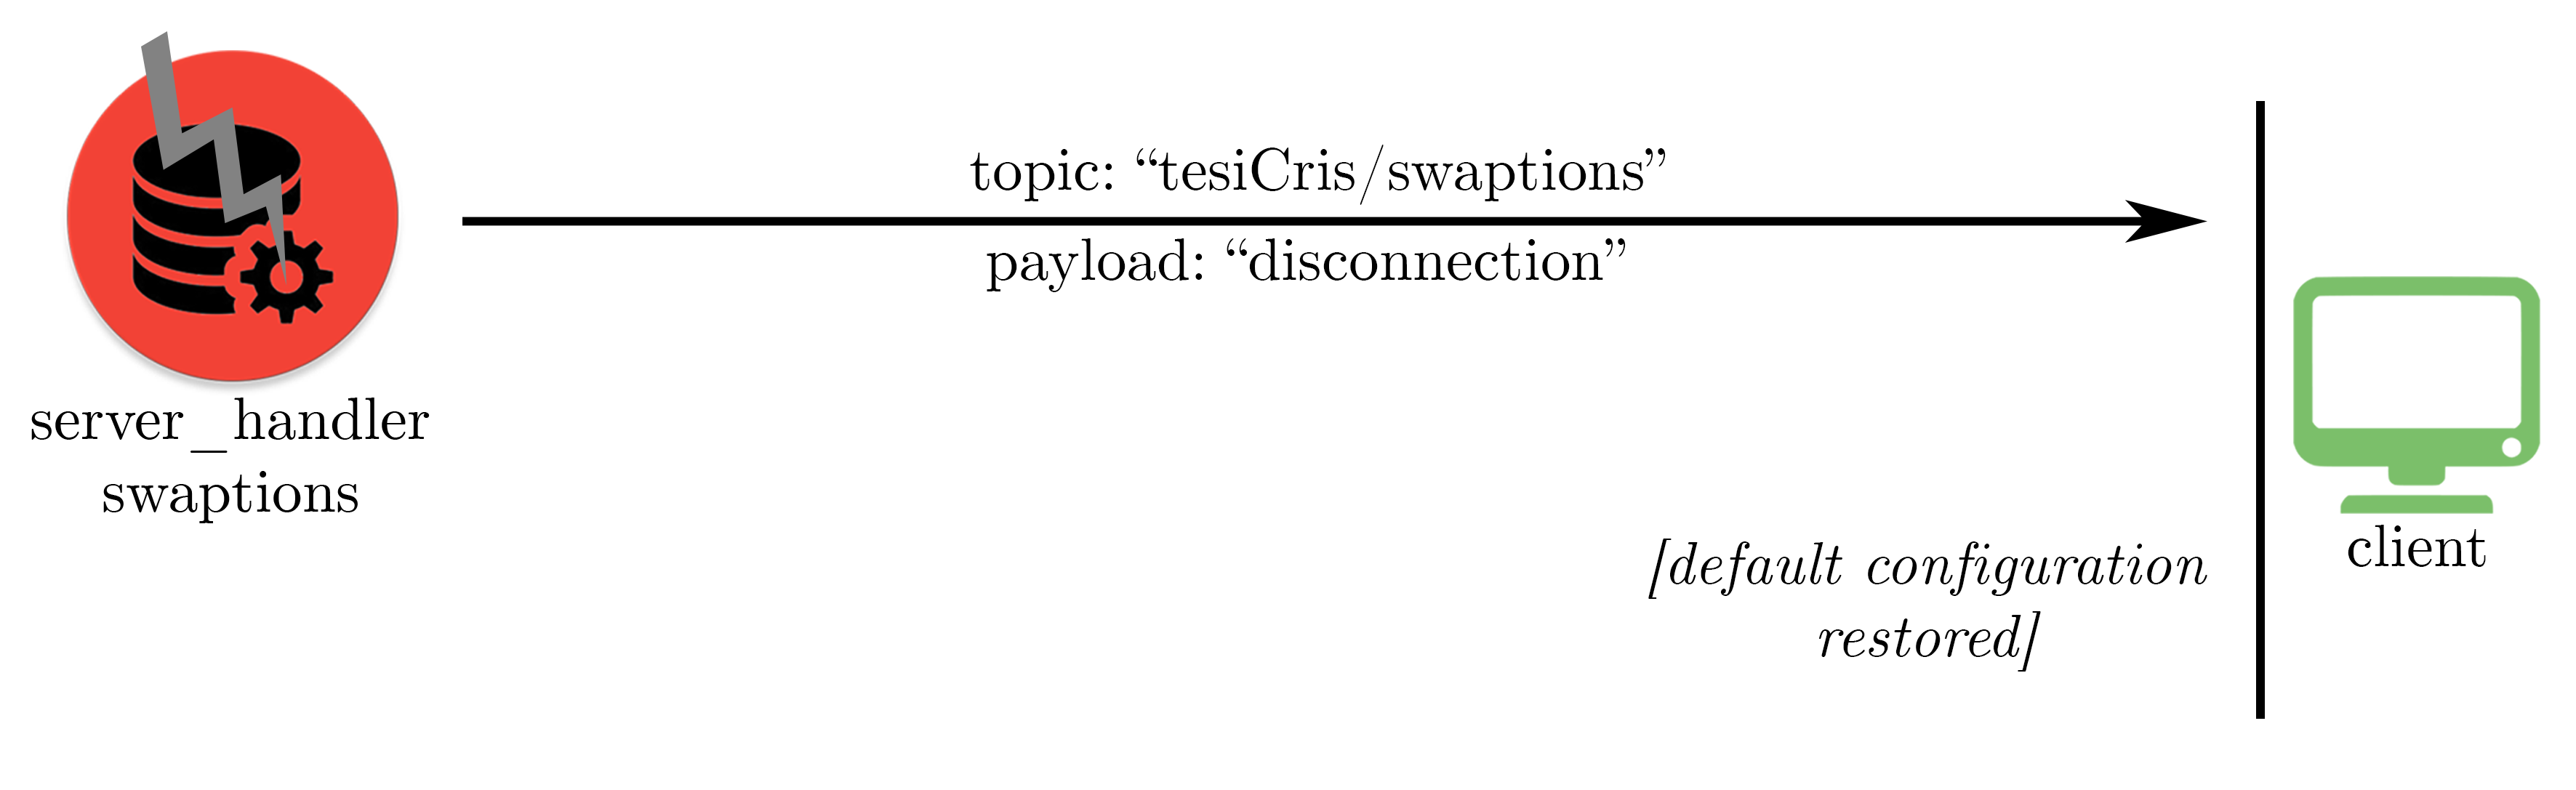
\includegraphics[width = \textwidth]{DSEinternal}
    \caption{server\_handler disconnection with client internal state equal to \textit{DSE} example}
    
\end{figure}


\subsubsection{client \textit{DoEModel} internal state}

Client has received a partial OP list, related to Design of Experiments configurations (see \ref{DoEModelSend}); in this case, the available OP list is not deleted, therefore the autotuner continues to work with this information.


\subsubsection{client \textit{autotuning} internal state}

Client has already received the predicted complete OP list from the server\_handler, therefore nothing changes.





\section{Client module integration}

\begin{figure}[H]

    \centering
    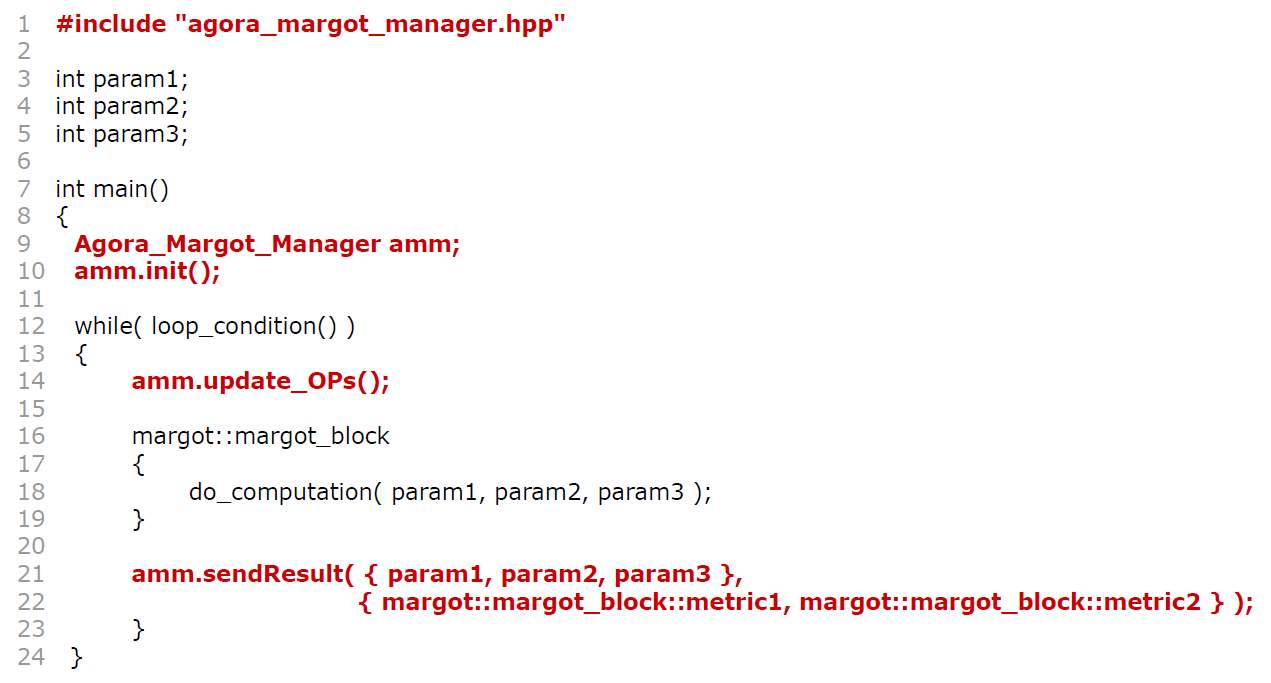
\includegraphics[width = \textwidth]{tesiCris_client_integration}
    \caption{Sketch application with \textit{AgoràLocalAppHandler} plus mARGOt autotuner integration}
    \label{fig::sketchApp}
    
\end{figure}

Figure \ref{fig::sketchApp} shows a sketch application that, until \textit{loop\_condition()} is verified (line 12), is executed; computation depends on three parameters (\textit{param1, param2, param3}) that are set up by mARGOt autotuner at the beginning of every cycle (line 16), while two metrics of interest (\textit{metric1, metric2}) are monitored (for mARGOt details, see the related scientific publication \cite{gadioli2015application}).

The integration code required to use tesiCris framework with mARGOt autotuner is written in bold red; three are the main steps during program execution:

\begin{enumerate}

    \item tesiCris client module and mARGOt autotuner instantiation and initialization (lines 9-10): the client module saves all application information and sets up mARGOt autotuner with a default Operating Point; if nothing happens, the application is executed with this configuration;
    
    \item Operating Points knowledge update (line 14): tesiCris module updates, from time to time, its internal knowledge about application configurations that are sent by the server\_handler; before mARGOt autotuner sets up application parameters (line 16), tesiCris checks mARGOt knowledge with respect to its internal one: if they are different, mARGOt configurations are updated. In this way, for instance, if the client module receives a new configuration during Design Space Exploration phase (see \ref{dse_conf}), mARGOt knowledge is set up with this data, so the application is forced to be executed with the corresponding parameters values; if, for instance, the complete model is received (see \ref{modelSend}), mARGOt internal knowledge is set up with all this information, so the autotuner can choose the best Operating Point that fulfils application current goals and requirements;
    
    \item Operating Point dispatch (line 21-22): after the computation has done, parameters values just used with the corresponding monitored metrics of interest are published on a predetermined MQTT topic, so the server\_handler that is in charge of this application can receive this information (see \ref{opSend}).
    
\end{enumerate}
